%% Submissions for peer-review must enable line-numbering
%% using the lineno option in the \documentclass command.
%%
%% Preprints and camera-ready submissions do not need
%% line numbers, and should have this option removed.
%%
%% Please note that the line numbering option requires
%% version 1.1 or newer of the wlpeerj.cls file, and
%% the corresponding author info requires v1.2

\documentclass[fleqn,10pt,lineno]{wlpeerj} % for journal submissions
% \documentclass[fleqn,10pt]{wlpeerj} % for preprint submissions

\newcommand{\cheng}[1]{\textcolor{orange}{\textbf{Cheng: }{\footnotesize #1}}}
\newcommand{\alasdair}[1]{\textcolor{blue}{\textbf{Alasdair: }{\footnotesize #1}}}

\usepackage{bm} % bold math symbols
\usepackage{hyperref} % create hyperlinks
\usepackage[labelfont=bf]{caption} % figure captions
\usepackage{subcaption}
\usepackage[boxed]{algorithm2e} % provide environment and layout to write pseudo-code
\usepackage{IEEEtrantools} % more flexible formatting of equations
\usepackage{mathtools} % use DeclarePairedDelimiterXPP
\usepackage{etoolbox}
\hypersetup{
	colorlinks   = true, % Colours links instead of ugly boxes
	citecolor    = {blue},
	pdfauthor    = {Alasdair Tran and Cheng Soon Ong},
	pdftitle	 = {Combining Active Learning Suggestions},
}

\DeclareMathAlphabet{\mathcal}{OMS}{cmsy}{m}{n} % reset calligraphy font

% some convenient symbols
\DeclareMathOperator{\Beta}{Beta}
\DeclareMathOperator{\Bin}{Bin}
\DeclareMathOperator{\tr}{tr}
\newcommand{\A}{\mathpzc{A}}
\newcommand{\B}{\mathcal{B}}
\newcommand{\X}{\mathcal{X}}
\newcommand{\Y}{\mathcal{Y}}
\newcommand{\Ecal}{\mathcal{E}}
\newcommand{\Normal}{\mathcal{N}}
\newcommand{\Unlabelled}{\mathcal{U}}
\newcommand{\Labelled}{\mathcal{L}}
\newcommand{\R}{\mathcal{R}}
\newcommand*{\argmin}{\operatornamewithlimits{arg\,min}\limits}
\newcommand*{\argmax}{\operatornamewithlimits{arg\,max}\limits}
\newcommand{\MPBA}{\text{MPBA}}
\newcommand{\passive}{\text{passive}}
\newcommand{\Select}{\textsc{Select}}
\newcommand{\Update}{\textsc{Update}}
\newcommand{\bmu}{\bm{\mu}}
\newcommand{\bsigma}{\bm{\sigma}}
\newcommand{\btau}{\bm{\tau}}

% Expected value
\providecommand\given{}
\DeclarePairedDelimiterXPP\E[1]{\mathbb{E}}{[}{]}{}{
	\renewcommand\given{  \nonscript\:
		\delimsize\vert
		\nonscript\:
		\mathopen{}
		\allowbreak}
	#1
}
% Probability
\DeclarePairedDelimiterXPP\Prob[1]{\mathbb{P}}{(}{)}{}{
	\renewcommand\given{  \nonscript\:
		\delimsize\vert
		\nonscript\:
		\mathopen{}
		\allowbreak}
	#1
}

% Settings for algorithm blocks
\DontPrintSemicolon % don't display semicolons at the end of each line
\SetArgSty{textnormal} % no need to italicise
\SetKwProg{Fn}{function}{}{} % function keyword

% Number paragraphs that are followed by an equation with lineno properly
\newcommand*\patchAmsMathEnvironmentForLineno[1]{%
\expandafter\let\csname old#1\expandafter\endcsname\csname #1\endcsname
\expandafter\let\csname oldend#1\expandafter\endcsname\csname end#1\endcsname
\renewenvironment{#1}%
   {\linenomath\csname old#1\endcsname}%
   {\csname oldend#1\endcsname\endlinenomath}}%
\newcommand*\patchBothAmsMathEnvironmentsForLineno[1]{%
\patchAmsMathEnvironmentForLineno{#1}%
\patchAmsMathEnvironmentForLineno{#1*}}%
\AtBeginDocument{%
\patchBothAmsMathEnvironmentsForLineno{equation}%
\patchBothAmsMathEnvironmentsForLineno{align}%
\patchBothAmsMathEnvironmentsForLineno{IEEEeqnarray}%
}

\title{Combining Active Learning Suggestions}

\author[1]{Alasdair Tran}
\author[2, 3]{Cheng Soon Ong}
\author[3]{Christian Wolf}
\affil[1]{Research School of Computer Science, Australian National University}
\affil[2]{Machine Learning Research Group, Data61, CSIRO, Australia}
\affil[3]{Research School of Astronomy and Astrophysics, Australian National
          University}

\corrauthor[1]{Alasdair Tran}{alasdair.tran@anu.edu.au}

% \keywords{machine learning, active learning, bandit, rank aggregation,
%           expert advice, astronomy}

\begin{abstract}
We study the problem of combining active learning suggestions to identify
informative training examples in binary and multiclass classification.
Supervised machine learning relies on building a training set of labeled
examples, but this process is time-consuming as it requires manual annotation
from human experts. Many active learning heuristics have been proposed to help
us pick which instance to annotate next. But what is the optimal heuristic for
a particular problem? Motivated by the success of methods that combine
predictors, we propose to combine active learners with bandit algorithms and
rank aggregation methods. Using benchmark datasets, we demonstrate that there
is no need to pick a particular heuristic a priori, since we can cheaply
combine them without sacrificing the final accuracy.

\end{abstract}

\begin{document}

\flushbottom
\maketitle
\thispagestyle{empty}

\section{Introduction}
Recent advances in sensors and scientific instruments have led to an increasing
use of machine learning techniques for managing the data deluge. Supervised
learning has become a widely used paradigm in many big data applications.
However, labeled examples are required during the training phase of these
algorithms, and the labeling process has become a significant bottleneck.

The most common approach to produce a training set is passive learning, where
we randomly select an instance from a large pool of unlabeled data to annotate,
and we continue doing this until the training set reaches a certain size or
until the classifier makes sufficiently good predictions. Depending on how the
underlying data is distributed, this process can be quite inefficient. To see
why, consider two objects with very similar features. If we have already
labeled one of them, there would be little benefit in also labeling the other
object, especially if we assume that there is no noise in the label. Instead it
is often more informative to pick examples near the decision boundary of the
classifier, where the class membership is still uncertain.

This leads to the development of many active learning algorithms that try to
reduce the labeling bottleneck without sacrificing the classifier's
performance. This is done by actively choosing the most informative examples to
be labeled based on some predicted class probabilities.
Section~\ref{sec:heuristics} describes two families of algorithms in
detail---uncertainty sampling and version space reduction.

This paper presents a survey of how we can combine suggestions from various
heuristics. In supervised learning, combining predictors is a well-studied
problem. Many techniques such as AdaBoost~\citep{freund96} (which averages
predictions from a set of models) and decision trees~\citep{breiman84} (which
select one model for making predictions in each region of the input space) have
been shown to perform better than just using a single model. Inspired by this
success, we propose to combine active learning suggestions with bandit and
social choice theories in Section~\ref{sec:expert}. The use of bandit
algorithms, which pick one heuristic at each time step, has been studied
before~\citep{baram04, hsu15}. However, as far as we know, this is the first
time that social choice theory is used to rank and aggregate the suggestions.

To compare the algorithms, we run them on 11 benchmark datasets from the UCI
Machine Learning Repository and a large dataset from the Sloan Sky Digital Sky
Survey (SDSS). The experiment setup and discussion are described in
Section~\ref{sec:expt}. Our three main findings are: active learning is better
than passive learning; combining active learners does not in general degrade
the performance; and social choice theory provides more practical algorithms
than bandit theory since we do not need to design a reward scheme.


\section{Overview of Active Learning}~\label{sec:heuristics}
Consider the classification setting where we would like to learn a classifier
$h$, which is a function that maps some feature space $\X \subseteq
\mathbb{R}^d$ to a probability distribution over a finite label space $\Y$:
\begin{IEEEeqnarray}{lCl}
	h : \X \rightarrow p(\Y)
\end{IEEEeqnarray}
For example, in logistic regression with two classes, $\Y = \{0, 1\}$, we can
model the probability that an object with feature vector $\bm{x}$ belongs to
the positive class with
\begin{IEEEeqnarray}{lCl}
	h(\bm{x}; \bm{w}) &=& p(1 \mid \bm{x}; \bm{w})
	= \dfrac{1}{1 + e^{-\bm{w}^T \bm{x}}}
\end{IEEEeqnarray}
and the training process involves learning the optimal weight vector $\bm{w}$.

In pool-based active learning, where we select an object from a pool of
unlabeled examples at each time step, we also require that some objects have
already been labeled initially. In practice, this normally means that we label
a small random sample at the beginning. These become the labeled set
$\Labelled_T \subset \X \times \Y$, and the rest form the unlabeled set
$\Unlabelled \subset \X$. Finally we also need a separate test set $\Labelled_S
\subset \X \times \Y$, which allows us to see how well the model generalizes
to unseen data.

Now consider the problem of choosing the next example in $\Unlabelled$ for
querying. Labeling can be a very expensive task, perhaps because it requires
actual human experts to manually examine each object. Thus we want to be smart
in choosing the next example. This motivates us to come up with a rule
$r(\bm{x}; h)$ that gives each unlabeled example a score based only on their
feature vector $\bm{x}$ and the current classifier $h$. In particular, we use
the probability estimates from the classifier over the unlabeled examples to
calculate the scores:
\begin{IEEEeqnarray}{lCl}
	r : p(\Y)^{U} \rightarrow \mathbb{R}^{U}
\end{IEEEeqnarray}
where $U$ is the size of the unlabeled set $\Unlabelled$. Coupled with each
rule is an objective function $s$ that picks the most informative example
for labeling based on the scores:
\begin{IEEEeqnarray}{lCl}
	s : \mathbb{R}^{U} \rightarrow J_\Unlabelled
\end{IEEEeqnarray}
where $J_\Unlabelled$ is the index set over the unlabeled instances. The rule
can be as simple as an argmax or argmin function, depending on how the scores
are interpreted. Algorithm~\ref{alg:active} outlines the standard pool-based
active learning setting. Note that in practice, there can be a large amount of
unlabeled data, so for computational reasons, we only assign a score to a small
random sample of size $E$ from the unlabeled pool.

\begin{algorithm}[htbp]
	\KwIn{
    	unlabeled set $\Unlabelled$,
        labeled training set $\Labelled_T$,
        classifier $h(\bm{x})$,
        desired training size $n$,
        query size $E$,
        and active learning rule $r(\bm{x}; h)$.
        }
    \BlankLine
	\While{$|\Labelled_T| < n$}{
		Select a random sample $\Ecal$ of size $E$ from $\Unlabelled$. \;
		Select the most informative candidate $\bm{x}_*$ from $\Ecal$ using the
			active learning rule $r(\bm{x}; h)$. \;
        Ask the expert to label $\bm{x}_*$. Call the label $y_*$. \;
		Add the new labeled example to the training set:
			$\Labelled_T \leftarrow \Labelled_T  \cup (\bm{x}_*, y_*)$. \;
		Remove the new labeled example from the unlabeled set:
			$\Unlabelled \leftarrow \Unlabelled \setminus \bm{x}_*$. \;
        Retrain the classifier $h(\bm{x})$. \;
    }

	\caption{The pool-based active learning algorithm}
	\label{alg:active}
\end{algorithm}

Coming up with an optimal rule is itself a difficult problem, but there have
been many attempts to derive good heuristics. Five common ones, which we shall
use in the experiments, are described in Section~\ref{subsec:uncertainty}
and~\ref{subsec:version}. They roughly fall into two categories: uncertainty
sampling and version space reduction. There are also heuristics that involve
minimizing the variance or maximizing the classifier certainty of the model
\citep{schein07}, but we do not consider them in this paper as they are
computationally inefficient in practice.

\subsection{Uncertainty Sampling}~\label{subsec:uncertainty}
\cite{lewis94} introduce the idea of uncertainty sampling, where we select the
instance whose class membership the classifier is least certain about. These
tend to be points that are near the decision boundary of the classifier.
Perhaps the simplest way to quantify uncertainty is~\cite{culotta05}'s least
confidence heuristic, where we pick the candidate whose most likely label the
classifier is most uncertain about:
\begin{IEEEeqnarray}{lCl}
	(s \circ r)(\bm{x}; h) &=& \argmax_{x \in \Unlabelled}
	\left\{ \max_{y \in \Y} p(y | \bm{x}; h) \right\}
\end{IEEEeqnarray}
A second option is to calculate the entropy \citep{shannon48}, which measures
the amount of information needed to encode a distribution. Intuitively, the
closer the class probabilities of an object are to random guessing, the higher
its entropy will be. This gives us the heuristic of picking the candidate with
the highest entropy of the distribution over the classes:
\begin{IEEEeqnarray}{lCl}
	(s \circ r)(\bm{x}; h) &=& \argmin_{x \in \Unlabelled}
	\left\{\sum_{y \in \Y} p(y | \bm{x}; h)
	\log \big[ p(y | \bm{x}; h) \big] \right\}
\end{IEEEeqnarray}
Finally we can pick the candidate with the smallest margin, which is defined as
the difference between the two highest class probabilities \citep{scheffer01}:
\begin{IEEEeqnarray}{lCl}
	(s \circ r)(\bm{x}; h) &=& \argmin_{x \in \Unlabelled}
	\left\{ \max_{y \in \Y} p(y | \bm{x}; h) -
	\max_{z \in \Y \setminus \{y\}} p(z | \bm{x}; h)  \right\}
\end{IEEEeqnarray}
Since the sum of all probabilities must be 1, the smaller the margin is, the
more uncertain we are about the object's class membership.

\subsection{Version Space Reduction}~\label{subsec:version}
Instead of focussing on the uncertainty of individual predictions, we could
instead try to constrain the size of the version space, thus allowing the
search for the optimal classifier to be more precise. The version space is
defined as the set of all possible classifiers that are consistent with the
current training set. To quantify the size of this space, we can train a
committee of $B$ classifiers, $\B = \{h_1, h_2, ..., h_B\}$, and measure the
disagreement among the members about an object's class membership. Ideally,
each member should be as different from the others as possible but still be
still in the version space \citep{melville04}. In order to have this diversity,
we give each member only a subset of the training examples. Since there might
not be enough training data, we need to use bootstrapping and select samples
with replacement. Hence this method is often called Query by Bagging (QBB).

One way to measure the level of disagreement is to calculate the margin using
the class probabilities estimated by the committee \citep{melville04}:
\begin{IEEEeqnarray}{lCl}
	(s \circ r)(\bm{x}; h) &=& \argmin_{x \in \Unlabelled}
	\left\{ \max_{y \in \Y} p(y | \bm{x}; \B) -
	\max_{z \in \Y \setminus \{y\}} p(z | \bm{x}; \B)  \right\}
\end{IEEEeqnarray}
This looks similar to one of the uncertainty sampling heuristics, except now we
first average out the class probabilities predicted by the members before
minimizing the margin.~\cite{mccallum98} offer an alternative disagreement
measure which involves picking the candidate with the largest expected
Kullback-Leibler (KL) divergence from the average:
\begin{IEEEeqnarray}{lCl}
	(s \circ r)(\bm{x}; h) &=& \argmax_{x \in \Unlabelled}
	\left\{ \dfrac{1}{B}
	\sum_{b=1}^B D_{\mathrm{KL}}(p_b\|p_\B) \right\}
\end{IEEEeqnarray}
where $D_{\mathrm{KL}}(p_b\|p_\B)$ is the KL divergence from the probability
distribution that is averaged across the committee $\B$, to the distribution
predicted by a member $b \in \B$.

For convenience, we summarize the five heuristics discussed above in
Table~\ref{tab:heuristics}.

\begin{table}[h]
	\caption {Summary of active learning heuristics used in our experiments.
			  Notations: $p(y | \bm{x}; h)$ is the probability of that an object
			  with feature vector $\bm{x}$ has label $y$ under classifier $h$,
			  $\B$ is the set of $B$ classifiers $\{h_1, h_2, ..., h_B\}$, $\Y$
			  is the set of possible labels, $\Unlabelled$ is the set of
			  unlabeled instances, $D_{\mathrm{KL}}(p\|q)$ is the
			  Kullback-Leibler divergence of $p$ from $q$, and $p_\B$ is the
			  average prediction distribution of $\B$. For simplicity,
			  for heuristics that use minimization, we flip the sign of the
			  score so that we can always take the argmax to get the best
			  candidate.}
	\label{tab:heuristics}
	\centering
	\begin{tabular}{lll}
		\toprule
		{Active Learning Heuristic}  &  Objective Function  \\
		\midrule
        Least Confidence &
			$\argmax_{x \in \Unlabelled}
			\left\{ \max_{y \in \Y} p(y | \bm{x}; h) \right\}$ \\
		Highest Entropy &
			$\argmax_{x \in \Unlabelled} \left\{-\sum_{y \in \Y} p(y | \bm{x}; h)
            \log \big[ p(y | \bm{x}; h) \big] \right\}$
			\\[2ex]
		Smallest Margin &
			$\argmax_{x \in \Unlabelled} - \left\{ \max_{y \in \Y} p(y | \bm{x}; h) -
            \max_{z \in \Y \setminus \{y\}} p(z | \bm{x}; h)  \right\}$
			\\[2ex]
		Smallest QBB Margin &
			$\argmax_{x \in \Unlabelled} - \left\{ \max_{y \in \Y} p(y | \bm{x}; \B) -
            \max_{z \in \Y \setminus \{y\}} p(z | \bm{x}; \B)  \right\}$
			\\[2ex]
		Largest QBB KL &
			$\argmax_{x \in \Unlabelled} \left\{ \dfrac{1}{B}
               \sum_{b=1}^B D_{\mathrm{KL}}(p_b\|p_\B) \right\}$
			\\
		\bottomrule
	\end{tabular}
\end{table}

\section{Combining Suggestions with Expert Advice}~\label{sec:expert}
Out of the five heuristics discussed, how do we know which one is the most
optimal one? There have been some attempts in the literature to do a
theoretical analysis. Proofs are however scarce, and when there is one
available, they normally only work under restricted assumptions. For example,
\cite{freund97} show that the query by committee algorithm (a slight variant of
our two QBB heuristics) guarantees an exponential decrease in the prediction
error with the training size, but only when there is no noise. However, whether
any of these heuristics is guaranteed to beat passive learning is still an open
question.

This leads us to a more general problem of whether we can learn the optimality
by just looking at the predictions given by the heuristics. Let us frame this
as the problem of prediction with expert advice. Consider the heuristics as a
collection of $R$ experts, $\R = \{r_1, r_2, ..., r_R\}$. How each expert comes
up with the prediction is not important. At every step $t$, however, we
have the ability to ask each expert $r_i$ for a prediction, either of the next
most informative instance in the unlabeled pool, or a rank on all the unlabeled
instances. Our task now is to use this information, along with the history of
rewards in the case of bandits, to choose the best candidate. In the standard
setting, the environment would reveal the correct answer after we have made our
choice, but this is not available in our case. Instead, we only have an option
of receiving a reward that indicates how good the choice is.

Let us consider two approaches of taking in expert advice. We can either
consider the advice of only one expert at each time step (with bandit
algorithms), or we can aggregate the advice of all the experts (with social
choice theory).

\subsection{Combining Suggestions with Bandit Theory}

First let us turn our attention to the multi-armed bandit problem in
probability theory. The colorful name originates from the situation where a
gambler stands in front of a slot machine with $R$ levers. When pulled, each
lever gives out a random reward according to some unknown distribution. The
goal of the game is to come up with a strategy that can maximize the gambler's
lifetime rewards while minimizing the number of pulls.

In the context of active learning, each lever is a heuristic with a different
ability to identify the candidate whose labeling information is most valuable.
Bandit algorithms do not need to know the internal workings of the heuristics,
but only the reward received from using a particular heuristic. Based on
the history of all the rewards, the bandit algorithm can decide on which
heuristic to pick next. Formally, we have
\begin{IEEEeqnarray}{lCl}
	b : [0, 1]^{R \times T} \rightarrow J_\R
\end{IEEEeqnarray}
where $b$ is the bandit algorithm, $[0, 1]$ is a normalized reward between
0 and 1, and $J_\R$ is the index set over the set of heuristics $\R$, and $T$
is the time horizon.

What would be an appropriate reward in this setting? One option is the
incremental increase in the performance of the test set after the candidate is
added to the training set. We assume that the heuristic rewards are independent
of each other. This is reasonable since the theories with which we use to
derive the heuristics are mostly unrelated.

The main problem in multi-arm bandits is the trade-off between exploring random
heuristics and exploiting the best heuristic so far. There are many situations
in which we find our previously held beliefs to be completely wrong. By
always exploiting, we could miss out on the optimal heuristic. On the other
hand, if we explore too much, it could take us a long time to reach the desired
accuracy.

There have been some attempts to combine active learning suggestions in the
literature.~\cite{baram04} use the EXP4 multi-armed bandit algorithm to
automate the selection process.~\cite{hsu15} study an improved version, EXP4.P,
along with importance weighting to estimate the rewards using only the training
set. In this paper, we will be more comprehensive by comparing four algorithms
that address this exploration-vs-exploitation problem: Thompson sampling,
OC-UCB, kl-OCB, and EXP3++.

Algorithm~\ref{alg:bandit} outlines how bandits can be used in pool-based
active learning. The only difference between the bandit algorithms lies in the
\textsc{Select} function that picks which heuristic to use and the
\textsc{Update} function that updates the algorithm's parameters when receiving
a new reward.

\begin{algorithm}[htbp]
	\KwIn{
    	unlabeled set $\Unlabelled$,
        labeled training set $\Labelled_T$,
        classifier $h$,
        desired training size $n$,
        query size $E$,
        set of active learning heuristics $\R$,
        and bandit algorithm $B$ with two functions \Select\,and \Update.
        }
    \BlankLine
	\While{$|\Labelled_T| < n$}{
		Select a heuristic $r_* \in \R$ according to \Select. \;
		Select a random sample $\Ecal$ of size $E$ from $\Unlabelled$. \;
		Select the most informative candidate $\bm{x}_*$ from $\Ecal$ using the
			heuristic $r(\bm{x}; h)$. \;
        Ask the expert to label $\bm{x}_*$. Call the label $y_*$. \;
		Add the new labeled example to the training set:
			$\Labelled_T \leftarrow \Labelled_T  \cup (\bm{x}_*, y_*)$. \;
		Remove the new labeled example from the unlabeled set:
			$\Unlabelled \leftarrow \Unlabelled \setminus \bm{x}_*$. \;
		Retrain the classifier $h(\bm{x})$. \;
		Run the updated classifier on the test set to compute the increase
			 in the performance $\delta$. \;
        Update the parameters of $B$ with \Update$(\delta)$. \;
    }
    \caption{Pool-based active learning with bandit theory}
    \label{alg:bandit}
\end{algorithm}

\subsubsection{Thompson Sampling}

The oldest bandit algorithm is Thompson sampling \citep{thompson33} which
solves the exploration-exploitation trade-off from a Bayesian perspective.

Let $\rho_i$ be the reward\index{reward} of heuristic $r_i \in \R$. Observe
that even with the optimal heuristic, there are still two sources of error.
First, there could be error during the labeling process that causes the
performance to decrease. In addition, even without label noise, the classifier
trained on finite data might not be the right one, so we still cannot score
perfectly due to having a poor $h$. Conversely, a bad heuristic might be able
to pick an informative candidate due to pure luck. Thus there is always a
certain level of randomness in the reward received. We assume these errors to
be normally distributed with mean $\nu_i$ and variance $\tau_i^2$:
	\begin{IEEEeqnarray}{lCl}
		(\rho_i \mid \nu_i) \sim \Normal(\nu_i, \tau_i^2)
	\end{IEEEeqnarray}

If we knew both $\nu_i$ and $\tau_i^2$ for all heuristics, the problem would
become trivially easy since we just need to always use the heuristic that has
the highest mean reward. In practice, we do not know $\nu_i$, so let us assume
that it itself follows a normal distribution:
	\begin{IEEEeqnarray}{lCl}
        \nu_i \sim \Normal(\mu_i, \sigma_i^2)
    \end{IEEEeqnarray}

To make the problem tractable, let us assume that the variance $\tau_i^2$ is a
known constant. The goal now is to find a good algorithm that can estimate
$\mu_i$ and $\sigma_i^2$.

We start with a prior knowledge of $\mu_i$ and $\sigma_i^2$ for each heuristic
$r_i$. So long as we do not choose anything stupid, e.g.\ a zero variance, our
choice of prior should not matter too much in the long run. Since initially we
do not have any information about the performance of each heuristic, the
appropriate prior value for $\mu_i$ is $0$, i.e.\ there is no evidence (yet)
that any of the heuristics offers an improvement to the performance.

In each round, we draw a random sample $\nu_i'$ from the normal distribution
$\Normal(\mu_i, \sigma_i^2)$ for each $i$ and select heuristic $r_*$ that has
the highest sampled value of the mean reward:
    \begin{IEEEeqnarray}{lCl}
        r_* = \argmax_{i} \nu_i'
    \end{IEEEeqnarray}
We then use this heuristic to assign scores to the candidates. The object that
is deemed to be the most informative is then added to the training set and the
classifier is retrained. Next we use the updated classifier to predict the
labels of objects in the test set. Let $\delta$ be the reward observed. We now
have a new piece of information that we can use to update our prior belief
about the mean $\mu_*$ and the variance $\sigma_*^2$ of $r_*$. Using Bayes'
theorem, we can show that the posterior distribution of the mean reward remains
normal,
	\begin{IEEEeqnarray}{lCl}
        (\nu_* \mid \rho_* = \delta) \sim \Normal (\mu_*', {\sigma'_*}^2)
    \end{IEEEeqnarray}
with the following new mean and variance:
    \begin{IEEEeqnarray}{lClllCl}
		\mu_*' &=& \frac{\mu_* \tau^2_* + \delta \sigma^2_*}{\sigma^2_* + \tau^2_*}
		&\qquad\qquad
        {\sigma'_*}^2 &=& \frac{\sigma^2_* \tau^2_*}{\sigma^2_* + \tau^2_*}
	\end{IEEEeqnarray}
Algorithm~\ref{alg:thompson} summarizes the \textsc{Select} and \textsc{Update}
functions used in Thompson sampling.
\SetKwFunction{SelectFn}{Select}%
\begin{algorithm}[htbp]
	\Fn{\Select()}{
		\For{$i \in \{1, 2, ..., R\}$}{
			$\nu_i' \leftarrow$ draw a sample from $\Normal(\mu_i, \sigma^2_i)$ \;
			}
		Select the heuristic with the highest sampled value: $r_* \leftarrow \argmax_{i} \nu_i'$ \;
	}
	\BlankLine
	\Fn{\Update($\delta$)}{
		$\mu_* \leftarrow \dfrac{\mu_* \tau^2_* + \delta \sigma^2_*}{\sigma^2_* + \tau^2_*}$
		$\qquad\qquad$
		$\sigma_*^2 \leftarrow \dfrac{\sigma^2_* \tau^2_*}{\sigma^2_* + \tau^2_*}$ \;
	}
	\caption{Thompson sampling with normally distributed rewards. Notations:
			$\R$ is the set of $R$ heuristics, $\bmu$ is the mean parameter of
			the average reward, $\bsigma^2$ is the variance parameter of the
			average reward, and $\btau^2$ is the variance parameter of the
			reward, and $\delta$ is the reward received.}
	\label{alg:thompson}
\end{algorithm}

\subsubsection{Upper Confidence Bounds}

 Next we consider the Upper Confidence Bound (UCB) algorithms which use the
principle of ``optimism in the face of uncertainty''. In choosing which
heuristic to use, we first estimate the upper bound of the reward (that is, we
make an optimistic guess) and pick the one with the highest bound. If our guess
turns out to be wrong, the upper bound of the chosen heuristic will decrease,
making it less likely to get selected in the next iteration.

There are many different algorithms in the UCB family, e.g. UCB1-TUNED \& UCB2
\citep{auer02finite}, V-UCB \citep{audibert09}, OC-UCB \cite{lattimore15}, and
kl-UCB \citep{cappe13}. They differ only in the way the upper bound is
calculated. In this paper, we only consider the last two. In Optimally
Confident UCB (OC-UCB), \cite{lattimore15} suggests that we pick the heuristic
that maximizes the following upper bound:
    \begin{IEEEeqnarray}{lCl}
		r_* = \argmax_{i} \overline{\delta_i} +
			  \sqrt{\dfrac{\alpha}{T_i(t)} \ln\Big(\dfrac{\psi n}{t}\Big)}
    \end{IEEEeqnarray}
where $\overline{\delta_i}$ is the average of the rewards from $r_i$ that we
observe so far, $t$ is the time step, $T_i(t)$ is the number times we have
selected from heuristic $r_i$ before step $t$, and $n$ is the maximum number of
steps we are going take. There are two tunable parameters, $\alpha$ and $\psi$,
which the author suggests setting to 3 and 2, respectively.

\begin{algorithm}[htbp]
	\BlankLine
	\Fn{\Select()}{
		$r_* \leftarrow \argmax_{i} \overline{\delta_i} +
			  \sqrt{\dfrac{3}{T_i(t)} \ln\Big(\dfrac{2 n}{t}\Big)}$ \;
	}
	\BlankLine
	\Fn{\Update($\delta$)}{
		$t \leftarrow t + 1$ \;
		$T_*(t) \leftarrow T_*(t - 1) + 1$ \;
	}
	\caption{Optimally Confident UCB. Notations: $\R$ is the set of heursitics,
			 $n$ is the time horizon (maximum number of steps), $t$ is the
			 current time step, $T_i(t)$ counts of how many times heuristic $i$
			 has been selected, $\delta$ is the reward received, and
			 $\overline{\delta_i}$ is the average of the rewards from $r_i$ so
			 far.}
	\label{alg:oc-ucb}
\end{algorithm}


\cite{cappe13} suggests that we instead consider the KL-divergence when finding
to upper bound. In the case of normally distributed rewards with known variance
$\sigma^2$, the chosen heuristic would be
    \begin{IEEEeqnarray}{lCl}
		r_* = \argmax_{i} \overline{\delta_i} +
			  \sqrt{ 2 \sigma^2 \dfrac{\ln\big(T_i(t)\big)}{t} }
    \end{IEEEeqnarray}
Algorithm~\ref{alg:oc-ucb} and~\ref{alg:kl-ucb} summarize the these two OCB
approaches.

\begin{algorithm}[htbp]
	\BlankLine
	\Fn{\Select()}{
		$r_* \leftarrow \argmax_{i} \overline{\delta_i} +
				\sqrt{2 \sigma^2 \dfrac{\ln\big(T_i(t)\big)}{t}}$ \;
	}
	\BlankLine
	\Fn{\Update($\delta$)}{
		$t \leftarrow t + 1$ \;
		$T_*(t) \leftarrow T_*(t - 1) + 1$ \;
	}
	\caption{kl-UCB with normally distributed rewards. Notations: $\R$ is the
	set of heursitics, $\sigma$ is the variance of the rewards, $t$ is the
	current time step, $T_i(t)$ counts of how many times heuristic $i$ has been
	selected, $\delta$ is the reward received, and $\overline{\delta_i}$ is the
	average of the rewards from $r_i$ so far.}
	\label{alg:kl-ucb}
\end{algorithm}

\subsubsection{EXP3++}

The EXP3 algorithm was first developed by \cite{auer2002nonstochastic} to solve
the non-stochastic bandit problem where we make no statistical assumption about
the reward distribution. This is also often known as the adversarial setting,
where we have an adversary who generates an arbitrary sequence of rewards for
each heuristic in advance. We shall test~\cite{seldin14}'s EXP3++ algorithm
(see Algorithm~\ref{alg:exp3pp}). This is a generalization of the original
EXP3 and it has been shown to perform well in both the stochastic (where the
reward of each heuristic follows an unknown reward distribution) and
adversarial regime.

\begin{algorithm}[htbp]
	\BlankLine
	\Fn{\Select()}{
		$\beta = \dfrac{1}{2}\sqrt{\dfrac{\ln R}{t R}}$ \;
		\For{$i \in \{1, 2, ..., R\}$}{
			$\xi_i = \dfrac{18 \ln(t)^2}{t \min(1, \dfrac{1}{t} (L_i - \min(L)))^2}$ \;
			$\epsilon_i = \min\large(\dfrac{1}{2 R}, \beta, \xi_i \large)  $ \;
			$\rho_i = \dfrac{e^{-\beta * L_i}}{\sum_j e^{-\beta * L_j}}$ \;
			}
		$r_* \leftarrow \text{draw a sample from $\R$ with probabilities $\rho$}$ \;
	}
	\BlankLine
	\Fn{\Update($\delta$)}{
		$t \leftarrow t + 1$ \;
		$T_*(t) \leftarrow T_*(t - 1) + 1$ \;
		$L_* \leftarrow \dfrac{L_* + (1 - \delta)}{(1 - \sum_j \epsilon_j)
			   \rho_* + \epsilon_*} $
	}
	\caption{EXP3++ algorithm. Notations: $\R$ is the set of $R$ heursitics,
	$t$ is the current time step, $\beta$ is a parameter used to weight the
	heuristics for selection, $\xi_i$ and $\epsilon_i$ are used
	to compute the loss $L_i$, and $\delta$ is the reward received.}
	\label{alg:exp3pp}
\end{algorithm}

\subsection{Combining Suggestions with Social Choice Theory}

A drawback of the bandit methods is that at each iteration, we could only use
information from one particular suggestion. In addition, we also need to keep
around a test set, which is expensive and sometimes impossible to obtain in
practice. Since most suggestions require little computation, we could in fact
run all of them at the same time and then combine the rankings. This leads us
to social choice theory. Originally developed by political scientists like
Nicolas de Condorcet and Jean-Charles de Borda, this field of study is
concerned with how we aggregate preferences of a group of people to determine,
for example, the winner of an election~\citep{list13}. It has the nice property
that everyone (or in our context, every active learning heuristic) has a
voice.

For each heuristic $r_i$, we assign a score to every candidate like before. We
are not interested in the actual raw scores, but only in the relative ranking
$k(r_i)$ which converts the scores into a preference ordering:
	\begin{IEEEeqnarray}{lCl}
		k : \mathbb{R}^{U} \rightarrow \sigma(J_\Unlabelled)
	\end{IEEEeqnarray}
where $\sigma(J_\Unlabelled)$ is a permutation over the index set of the
unlabeled pool. $\Unlabelled$. An aggregation function $c$ will then combine
all the rankings into a combined ranking:
    \begin{IEEEeqnarray}{lCl}
		c : \sigma(J_\Unlabelled)^{|\R|} \rightarrow \sigma(J_\Unlabelled)
    \end{IEEEeqnarray}
From this, we can pick the highest-ranked candidate to label.

The central question in social choice theory is how we can come up with a good
preference aggregation rule. The main difference between this approach and the
bandit algorithms is that we do not consider the reward history when combining
the rankings, i.e.\ each heuristic is assumed to always have an equal weight. A
possible extension, which is not considered in this paper, is to use the past
performance to re-weight the heuristics before aggregating at each step.
Algorithm~\ref{alg:choice} provides an overview of how social choice theory is
used in pool-based active learning.

\begin{algorithm}[htbp]
	\KwIn{
    	unlabeled set $\Unlabelled$,
        labeled training set $\Labelled_T$,
        classifer $h$,
        desired training size $n$,
        query size $E$,
        set of active learning suggestions $\R$,
        and rank aggregator $G$.
        }
    \BlankLine
	\While{$|\Labelled_T| < n$}{
        $\Ecal$ $\leftarrow$ random sample of size $E$ from
            $\Unlabelled$ \;
        \For{$r \in \R$}{
        	Rank all the candidates in $\Ecal$. \;
        }
        Aggregate all the rankings into one ranking using $G$. \;
        $\bm{x}_* \leftarrow$ the highest ranked candidate in the aggregation. \;
        $y_* \leftarrow$ ask the expert to label $\bm{x}_*$ \;
        $\Labelled_T \leftarrow \Labelled_T  \cup (\bm{x}_*, y_*)$ \;
        $\Unlabelled \leftarrow \Unlabelled \setminus \bm{x}_*$ \;
        $h(\bm{x}) \leftarrow$ retrain the classifier \;
    }
    \caption{Pool-based active learning with social choice theory}
    \label{alg:choice}
\end{algorithm}

We shall examine three aggregation rules. In the most simple approach, Borda
count, we assign an integer point to each candidate. The lowest-ranked
candidate receives a point of 1, and each candidate receives one more point
than the candidate below. To aggregate, we simply add up all the points each
candidate receives from every heuristic. The candidate with the most points
is declared the winner and is to be labeled next.

We can think of Borda count, then, as ranking the candidate according to the
arithmetic mean. An alternative approach is to use the geometric mean
\citep{bedo14}, where instead of adding up the points, we multiply them.

The third approach we consider is the Schulze method~\citep{schulze11}. This
method is more computationally intensive since it requires examining all pairs
of candidates. In particular, we first compute the number of heuristics that
prefer candidate $i$ to candidate $j$. Let us call this $d(i, j)$. We then
define a path from candidate $i$ to $j$ as a sequence of candidates that starts
with $i$ and ends with $j$, where, as we move along the path, the number of
heuristics that prefer the current candidate over the next candidate must be
strictly decreasing. Intuitively, the path is the rank of a subset of
candidates, where $i$ is at the top and $j$ is at the bottom.

Associated with each path is a strength $p$, which is the minimum of $d(i, j)$
for all consecutive $i$ and $j$ along the path. Our task, then, is to find the
path of the strongest strength from each candidate to every other. This problem
has a similar flavour to the problem of finding the shortest path. In fact, the
implementation uses a variant of the Floyd–Warshall algorithm to find the
strongest path. This is the most efficient implementation that we know of,
taking quadratic time in the number of candidates.

We end this section with a small illustration of how the three aggregation
algorithms work in Table~\ref{tab:choice}.

\begin{table}[htbp]
	\caption {An example of how social choice theory algorithms rank four
	          candidates by aggregating three heuristics: $r_1$, $r_2$, and
	          $r_3$. The unlabeled pool consists of four objects: A, B, C, and
	          D.} \label{tab:choice}
	\centering
	\begin{subtable}{\linewidth}
		\centering
		\begin{tabular}{lrrrr}
			\toprule
			{Heuristic}  &  Ranking \\
			\midrule
				$r_1$ & B A C D \\
				$r_2$ & A C B D \\
				$r_3$ & B D C A \\
			\bottomrule
		\end{tabular}
		\caption{An example of how the three heuristics rank four candidates $A, B, C, D$.}
	\end{subtable}

	\begin{subtable}{\linewidth}
		\centering
		\begin{tabular}{lrrrr}
			\toprule
			{Candidate}  &  Borda count & Geometric mean \\
			\midrule
				A & $3 + 4 + 1 = 8$ & $3 * 4 * 1 = 12$ \\
				B & $4 + 2 + 4 = 10$ & $4 * 2 * 4 = 32$ \\
				C & $2 + 3 + 2 = 7$ & $2 * 3 * 2 = 12$ \\
				D & $1 + 1 + 3 = 5$ & $1 * 1 * 3 = 3$ \\
			\bottomrule
		\end{tabular}
		\caption{Aggregated ranking with Borda count and geometric mean: In both
		methods, candidate B receives the highest aggregated score.}
	\end{subtable}

	\begin{subtable}{\linewidth}
		\centering
		\begin{tabular}{lrrrr}
			\toprule
			{From / To}  & A & B & C & D \\
			\midrule
				A &   & 1 & 2 & 2 \\
				B & 2 &   & 2 & 3 \\
				C & 1 & 1 &   & 2 \\
				D & 2 & 0 & 1 &   \\
			\bottomrule
		\end{tabular}
		\caption{Aggregated ranking with Schulze method: We show the strongest
		path strengths $p(i, j)$ between all pairs of candidates. Candidate B
		is the winner since $p(B, A) > p(A, B)$, $p(B, C) > p(C, B)$, and $p(B,
		D) > p(D, B)$.}
	\end{subtable}
\end{table}


\section{Experiments}\label{sec:expt}

\subsection{Description of datasets}

We use 11 datasets taken from the UCI Machine Learning
Repository~\citep{lichman13}, along with one large dataset SDSS from the
astronomical domain \citep{alam15}. Table~\ref{tab:datasets} shows the size and
the number of classes in each dataset, along with the proportion of the samples
belonging to the majority class and the maximum achievable performance.

\begin{table}[htbp]
	\caption {Overview of datasets} \label{tab:datasets}
	\centering
	\begin{tabular}{lrrrrr}
		\toprule
		{Dataset}  & Size &  Classes & Features & Majority & Max MPBA \\
		\midrule
        \href{https://archive.ics.uci.edu/ml/datasets/Glass+Identification}{glass}
        	& $214$ & $6$ & $10$ & $33\%$ & $65\%$ \\
		\href{https://archive.ics.uci.edu/ml/datasets/Ionosphere}{ionosphere}
			& $351$ & $2$ & $34$ & $64\%$ & $89\%$ \\
		\href{https://archive.ics.uci.edu/ml/datasets/Iris}{iris}
        	& $150$ & $3$ & $4$ & $33\%$ & $90\%$ \\
        \href{https://archive.ics.uci.edu/ml/datasets/MAGIC+Gamma+Telescope}{magic}
        	& $19~020$ & $2$ & $11$ & $65\%$ & $84\%$ \\
        \href{https://archive.ics.uci.edu/ml/datasets/MiniBooNE+particle+identification}{miniboone}
        	& $129~596$ & $2$ & $50$ & $72\%$ & $88\%$ \\
        \href{https://archive.ics.uci.edu/ml/datasets/Page+Blocks+Classification}{pageblock}
        	& $5~473$ & $5$ & $10$ & $90\%$ & $79\%$ \\
		\href{https://archive.ics.uci.edu/ml/datasets/Pima+Indians+Diabetes}{pima}
        	& $733$ & $2$ & $8$ & $66\%$ & $71\%$ \\
        \href{http://dx.doi.org/10.5281/zenodo.58500}{sdss}
        	& $2~801~002$ & $3$ & $11$ & $61\%$ & $90\%$ \\
		\href{https://archive.ics.uci.edu/ml/datasets/Connectionist+Bench+(Sonar,+Mines+vs.+Rocks)}{sonar}
        	& $208$ & $2$ & $60$ & $53\%$ & $78\%$ \\
        \href{https://archive.ics.uci.edu/ml/datasets/Statlog+(Vehicle+Silhouettes)}{vehicle}
			& $846$ & $4$ & $18$ & $26\%$ & $81\%$ \\
		\href{https://archive.ics.uci.edu/ml/datasets/Wine}{wine}
        	& $178$ & $3$ & $13$ & $40\%$ & $94\%$ \\
		\href{https://archive.ics.uci.edu/ml/datasets/Breast+Cancer+Wisconsin+(Prognostic)}{wpbc}
        	& $194$ & $2$ & $34$ & $76\%$ & $58\%$ \\
		\bottomrule
	\end{tabular}
\end{table}

\subsection{Experimental Setup}
For each dataset, we build a classifier with the classes being the output. We
use a 10-fold stratified shuffled split cross validation. The stratified
strategy means that the proportion of the classes remain constant in each
split. We standardise all features to have zero mean and unit variance.
Although all examples has already been labeled, we simulate active learning by
assuming that certain examples do not have any labels. In particular, the
unlabeled pool size is 70\% of data up to a maximum of 10,000 examples. The
test pool consists of the remaining examples up to a maximum of 20,000---we
assume labels are available here. We initialize the classifier by labeling 10
random samples and using them as the the initial training set. We use logistic
regression with a Gaussian kernel approximation and an L2 loss. In the binary
case, the loss function is
\begin{IEEEeqnarray}{lCl}
    L &=& \dfrac{1}{2} w^T w + C \sum_{i = 1}^n \ln\Big(1 + \exp(-y_i(f(X_i)^T w))\Big)
\end{IEEEeqnarray}
where the first term of the sum is the regularisation term to ensure that the
weight vector is not too large, and $C$ is another regularisation
hyperparameter which we set to 1000. To speed up training time, we approximate
the feature map of the Gaussian kernel using Random Kitchen Sinks
\citep{rahimi08}, transforming the raw features $X_i$ into a fixed
100-dimensional feature vector $f(X_i)$. In the multiclass case, we use the
One-vs-Rest strategy, where for every class, we build a binary classifier that
determines whether a particular example is in that class or not.

For the reward, we use the mean posterior balanced accuracy (MPBA) as the
reward. Compared to a simple accuracy rate, this measure takes into account the
class imbalance. Intuitively, we calculate the recall rate in each class and
then take the average, giving each class an equal weight. Refer to Appendix B
for the derivation of the MPBA.

Given that there are 12 datasets, each with 17 learning curves, we need a
measure that can summarize in one number how well a particular heuristic or
policy does. Building on~\cite{baram04}'s deficiency measure, we define the
strength of an active learner or policy, relative to passive learning, as
\begin{IEEEeqnarray}{lCl}
    \text{Strength}(h; m) &=&
    	1 - \dfrac{\sum_{t=1}^{n}\big(m(\max) - m(h, t)\big)}
    	{\sum_{t=1}^{n}\big(m(\max) - m(\passive, t)\big)}
\end{IEEEeqnarray}
where $m$ is a chosen metric (e.g. accuracy rate, F1-score, MPBA), $m(\max)$ is
the best possible performance achieved from using all labeled data in the
training set, and $m(h, t)$ is the performance achieved using the first $t$
examples selected by heuristic $h$. The summation can then be thought of as the
area between the best possible performance line and the learning curve of $h$.
The better the heuristic is, the faster it would approach this maximum line,
and thus the smaller the area. Finally, so that we can compare the performance
across datasets, we normalise the measure with the area obtained from using
just passive learning.

The abbreviations used when discussing the results are outlined in Table~\ref{tab:abbre}.

\begin{table}[htbp]
	\caption {Heuristics and Policies} \label{tab:abbre}
	\centering
	\begin{tabular}{ll}
		\toprule
		{Abbreviation}  & Description \\
		\midrule
        passive
        	& Passive learning \\
		confidence
			& Least confidence heuristic \\
		w-confidence
        	& Least confidence heuristic with information density weighting \\
        margin
        	& Smallest margin heuristic \\
        w-margin
        	& Smallest margin heuristic with information density weighting \\
        entropy
        	& Highest entropy heuristic \\
		w-entropy
        	& Highest entropy heuristic with information density weighting \\
        qbb-margin
        	& Smallest QBB margin heuristic \\
		qbb-kl
        	& Largest QBB KL-divergence heuristic \\
        explore
			& Bandit algorithm with 100\% exploration \\
		thompson
        	& Thompson sampling \\
		ocucb
			& Optimally Confidence UCB algorithm \\
		klucb
			& kl-UCB algorithm \\
		exp++
			& EXP3++ algorithm \\
		borda
			& Aggregation with borda count \\
		geometric
			& Aggergation with geometric mean \\
		schulze
			& Aggregation with Schulze method \\
		\bottomrule
	\end{tabular}
\end{table}

\section{Discussion}

Figures~\ref{fig:strengths-accuracy} to~\ref{fig:strengths-mpba} show the
strengths of all policies that we consider, while
Figures~\ref{fig:learning_curves-accuracy} to~\ref{fig:learning_curves-mpba}
provides the learning curves of a selected few. With the exception of the wpbc
dataset, most of the policies manage to beat passive learning. For the
individual heuristics, the least confidence seems to perform very well while
being very simple to calculate. This is consistent with have been observed in
the literature. The best performing bandit algorithm is EXP3++, and if we want
to use information form all heuristics, Borda count would be a good choice. On
some datasets such as magic and pima, Borda count does better than EXP3++,
although the effect is fairly small.

In practice, we do not have a representative test set that can be used to
compute the reward. Thus aggregation methods like Borda are are suitable than
bandit algorithms such as EXP3++ and Thompson sampling. In the absence of such
a test set, \cite{hsu15} addressed this problem by using importance weighting
to remove the bias in the accuracy on the training set. For this to work,
however, we need to ensure that every training example and active learning
suggestion have a non-zero probability of being selected in every iteration.

Finally, it is worth noting that active learning might degrade the classifier's
performance in some cases. This can be seen with the wpbc dataset, where no
policy manages to beat passive learning. This dataset does have the lowest
maximum performance, where we achieve an MPBA of only 58\% (slightly above
random guessing) when using the all examples in training. This indicates that
we would be better off with passive learning with datasets that are very noisy.

\begin{itemize}
	\item Additionally add ranking combination
	\item Active is better than passive
	\item Combining is better than single
	\item Bandit is the same as random combine, problem with reward design
\end{itemize}

\begin{figure}[tbp]
	\centering
	\begin{subfigure}[t]{\textwidth}
        \centering
        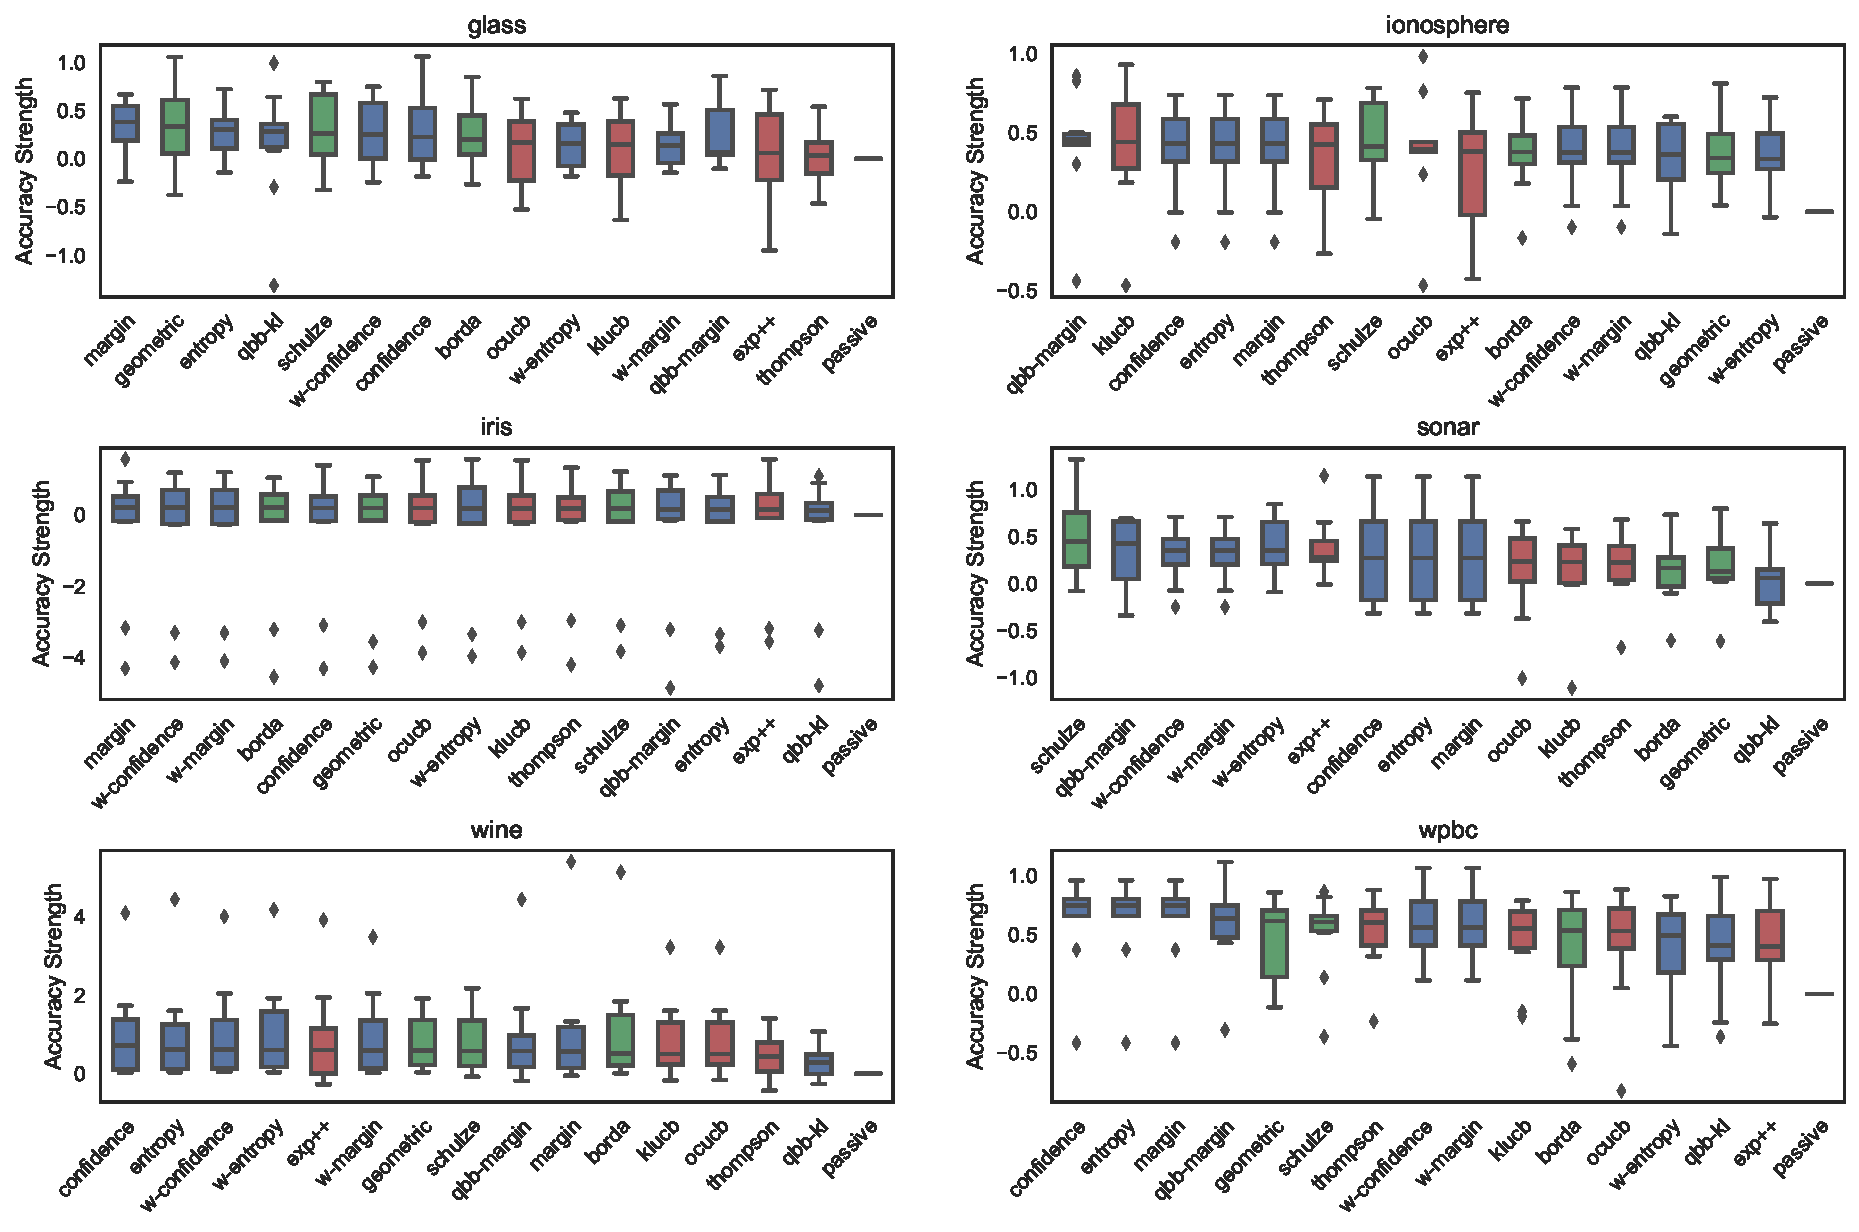
\includegraphics[width=\textwidth]{figures/strengths-accuracy-small}
        \caption{Small datasets}
	\end{subfigure}
	\begin{subfigure}[t]{\textwidth}
        \centering
        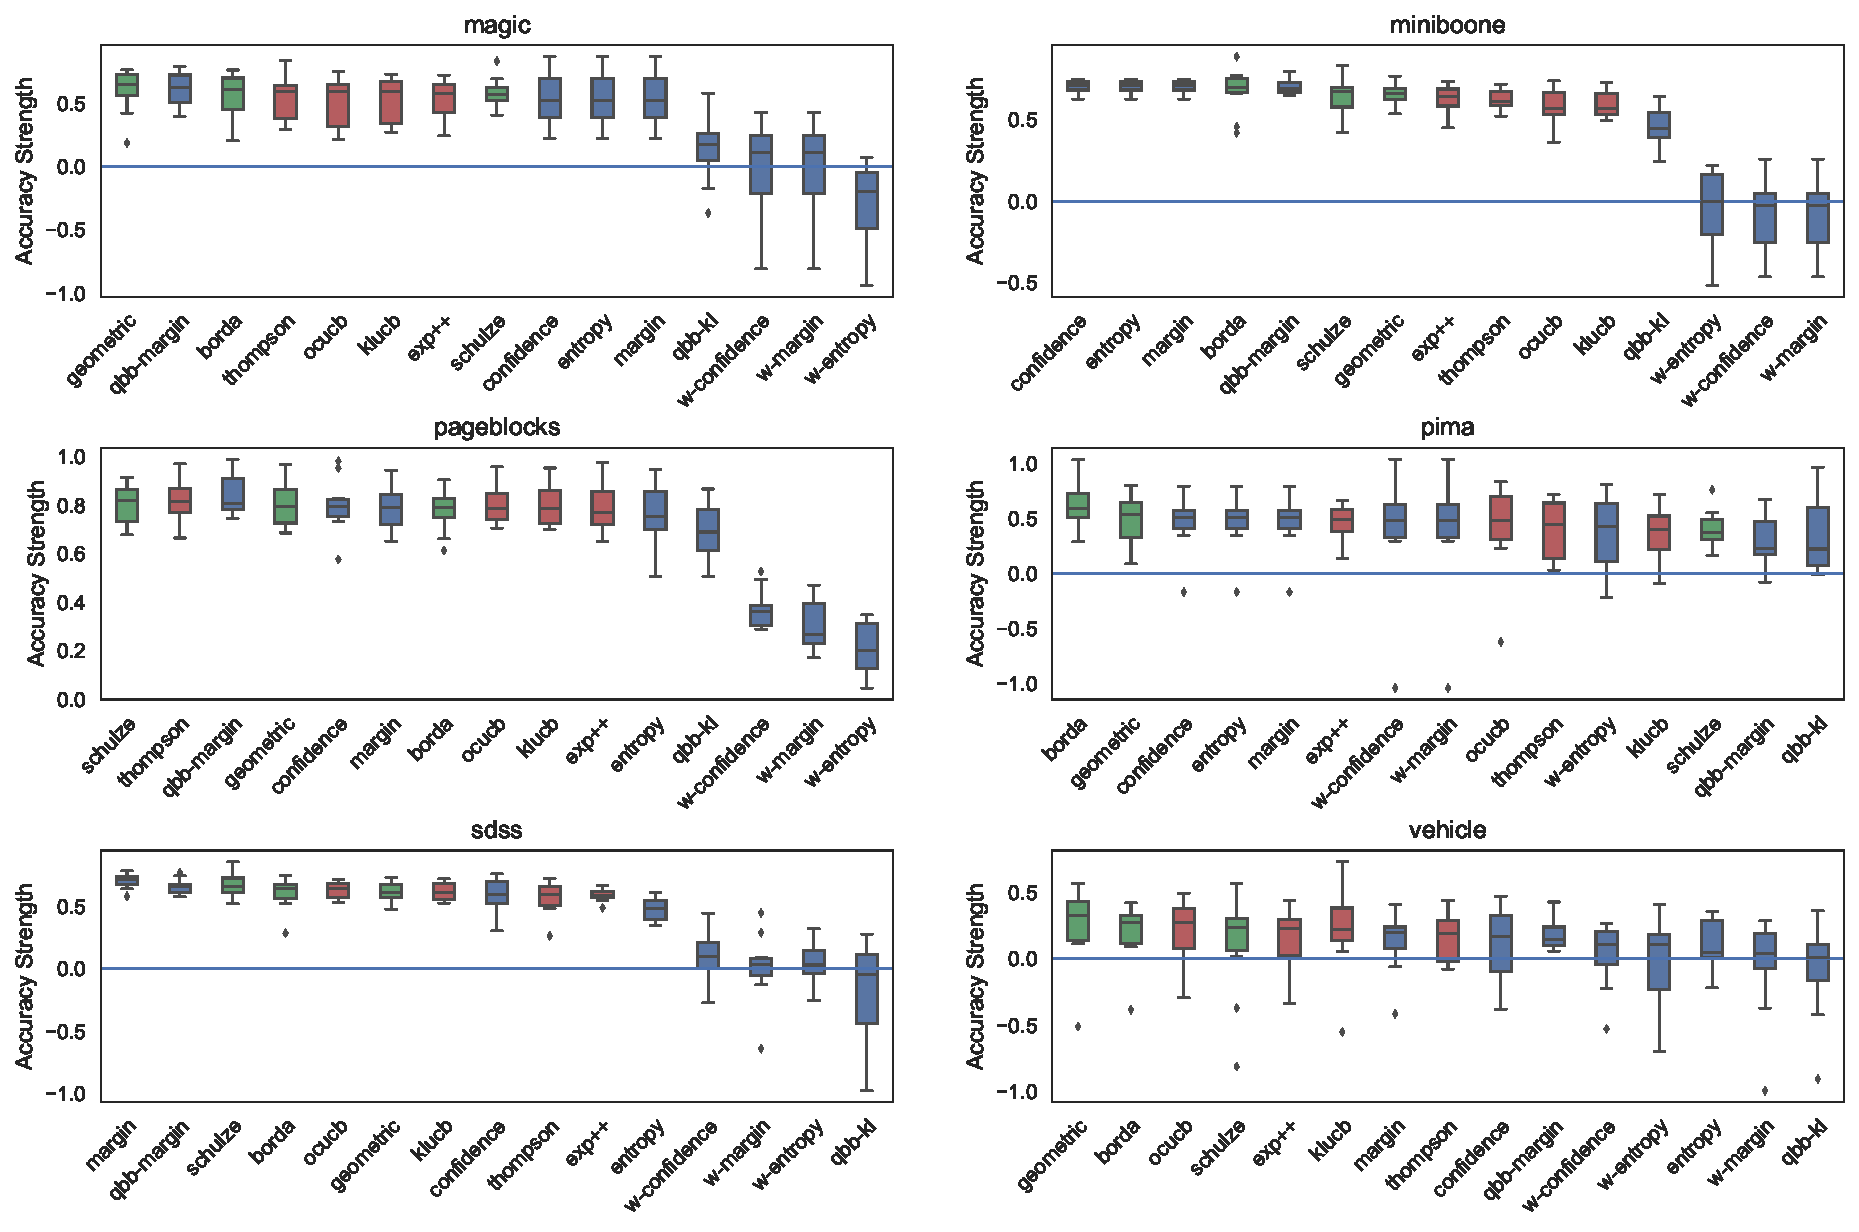
\includegraphics[width=\textwidth]{figures/strengths-accuracy-large}
        \caption{Large datasets}
    \end{subfigure}
	\caption[Policy strength]{Boxplots of accuracy strength of policies and
	heuristics relative to passive learning. The more positive the strength is,
	the better the heuristic/policy. Blue boxes represent individual
	heuristics; red boxes represent bandit alogrithms, and green boxes are for
	rank aggragation algorithms. Each plot is over 10 trials.}
	\label{fig:strengths-accuracy}
\end{figure}

\begin{figure}[tbp]
	\centering
	\begin{subfigure}[t]{\textwidth}
        \centering
        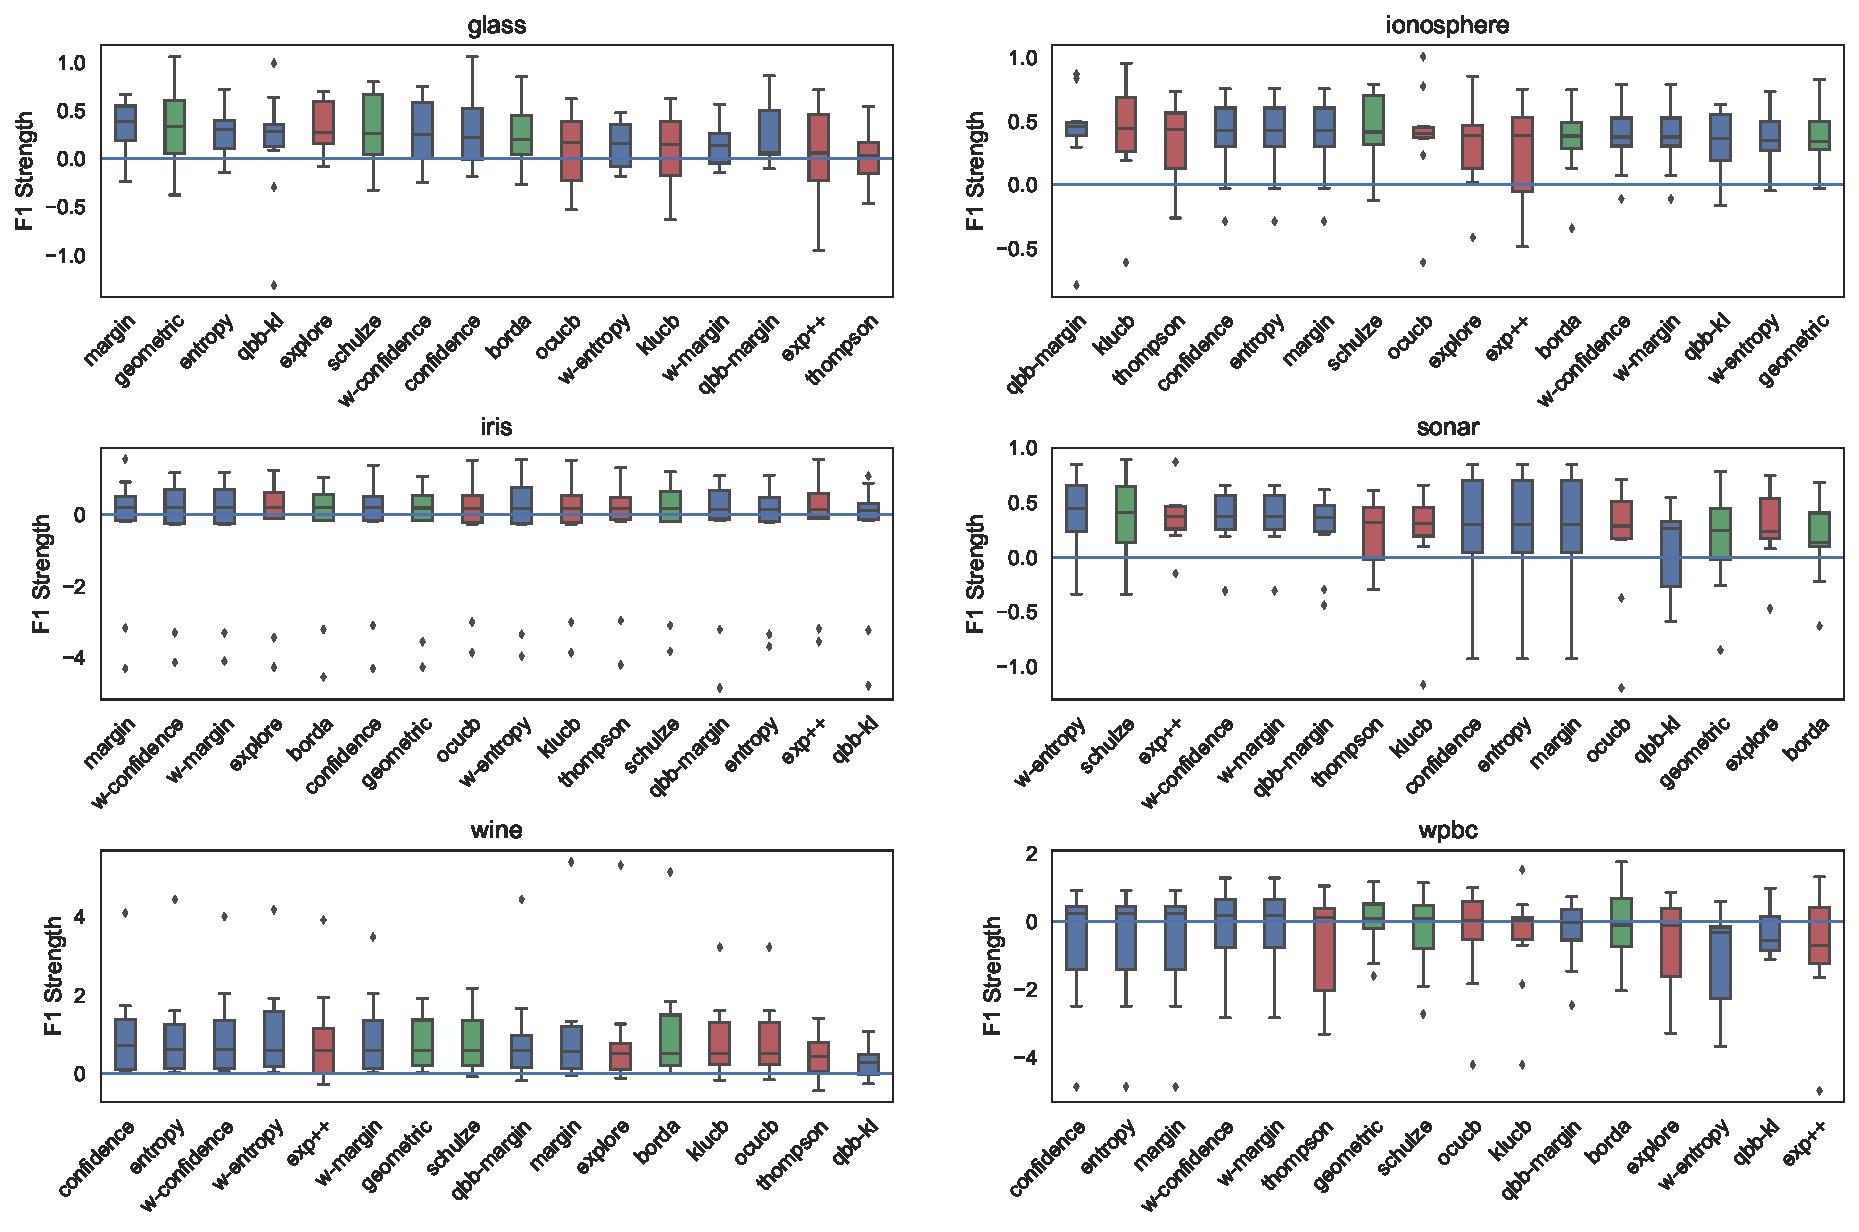
\includegraphics[width=\textwidth]{figures/strengths-f1-small}
        \caption{Small datasets}
	\end{subfigure}
	\begin{subfigure}[t]{\textwidth}
        \centering
        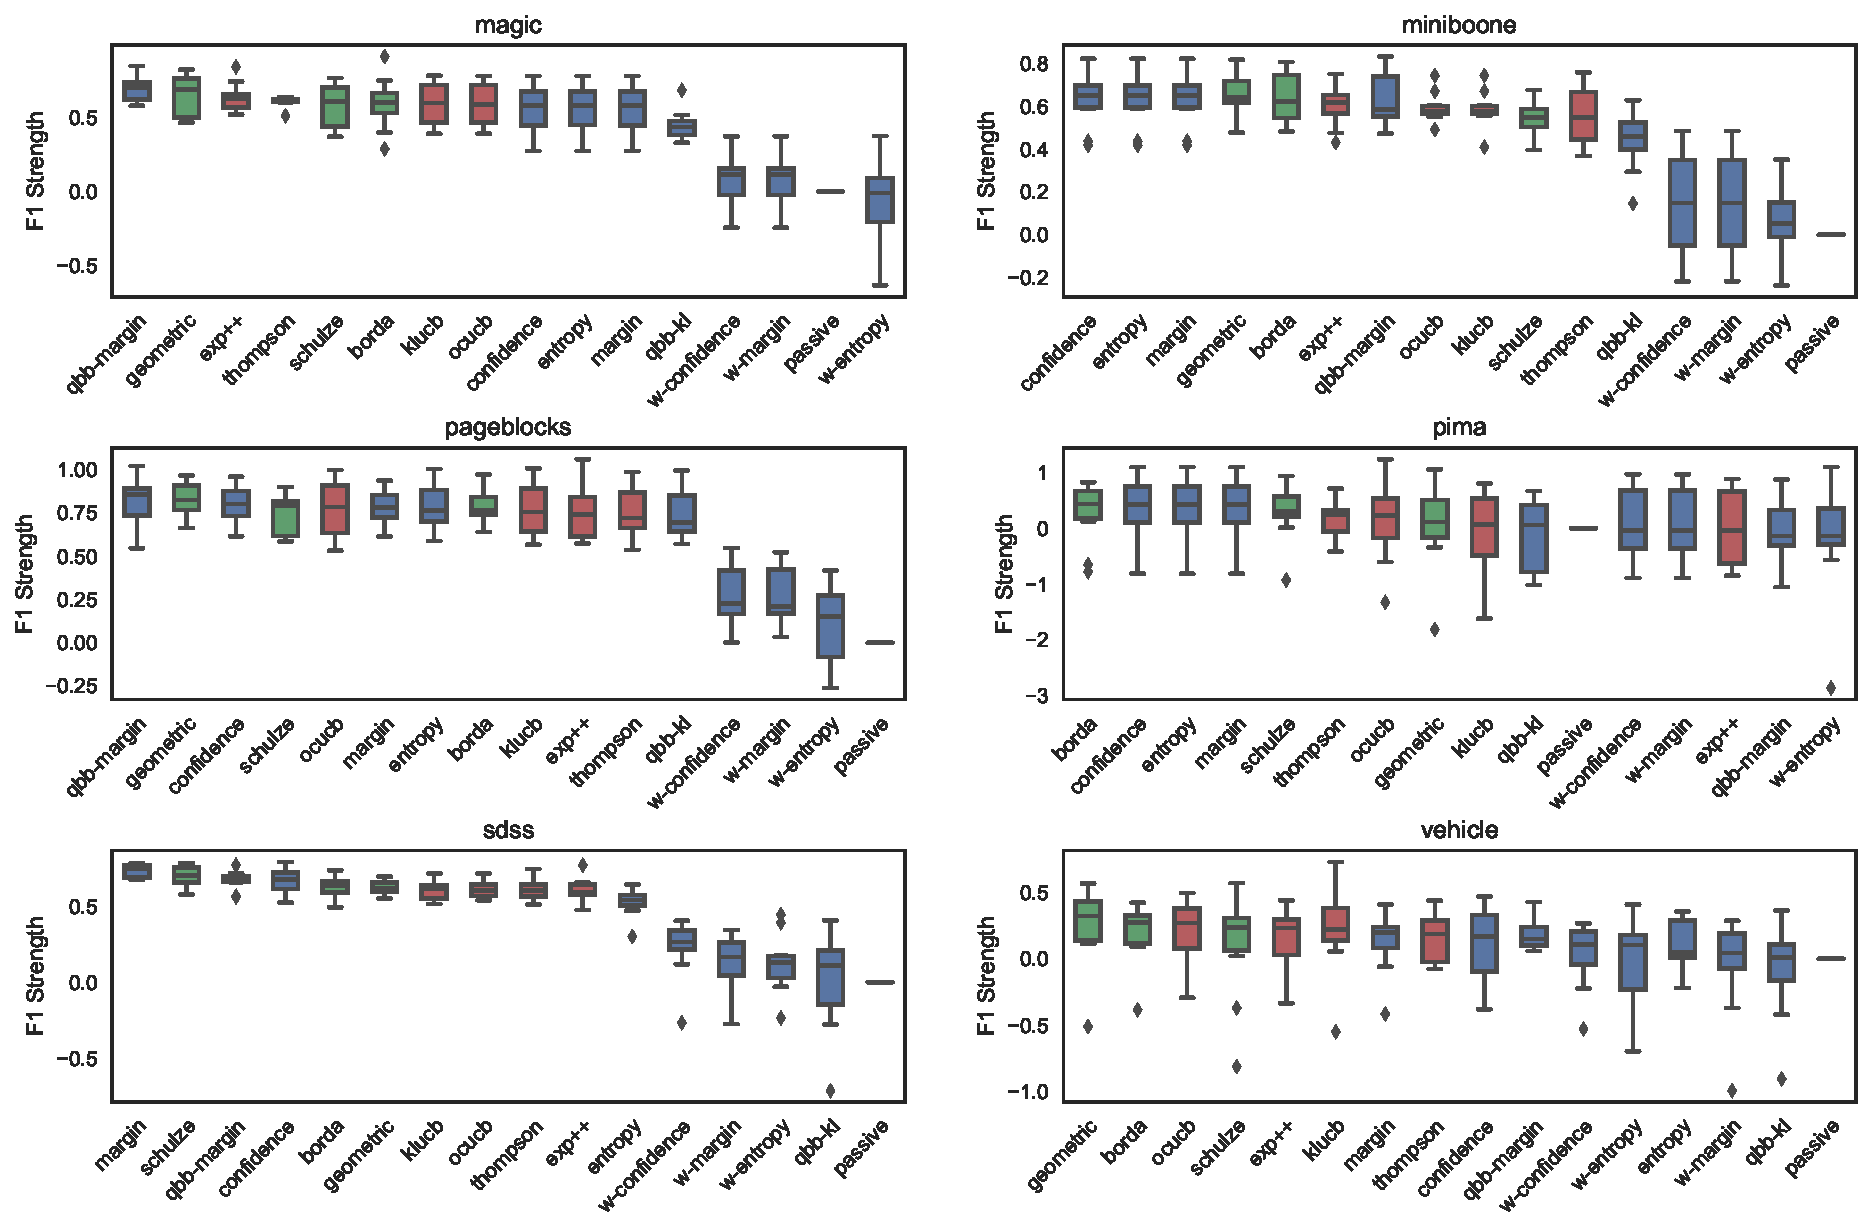
\includegraphics[width=\textwidth]{figures/strengths-f1-large}
        \caption{Large datasets}
    \end{subfigure}
	\caption[Policy strength]{Boxplots of F1 strength of policies and
	heuristics relative to passive learning. The more positive the strength is,
	the better the heuristic/policy. Blue boxes represent individual
	heuristics; red boxes represent bandit alogrithms, and green boxes are for
	rank aggragation algorithms. Each plot is over 10 trials.}
	\label{fig:strengths-f1}
\end{figure}

\begin{figure}[tbp]
	\centering
	\begin{subfigure}[t]{\textwidth}
        \centering
        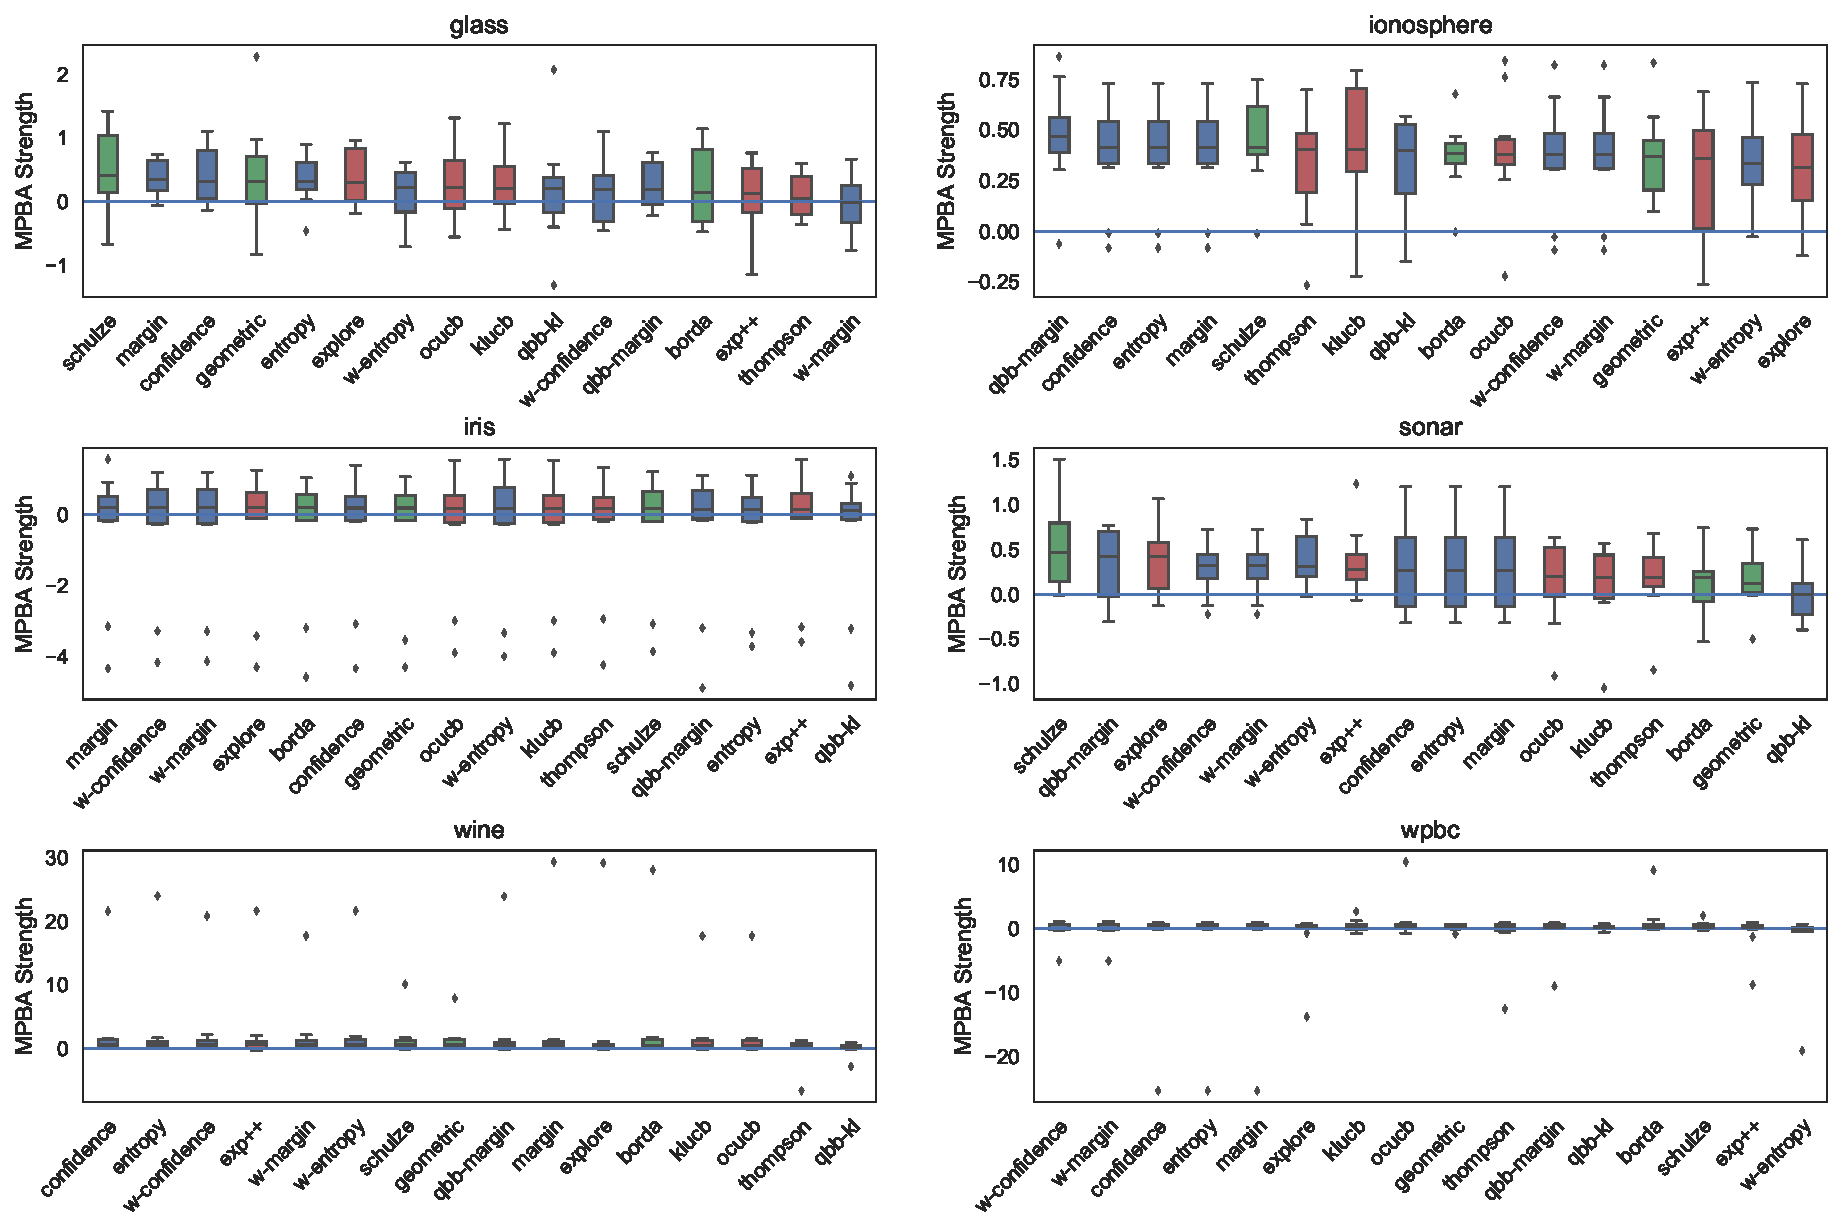
\includegraphics[width=\textwidth]{figures/strengths-mpba-small}
        \caption{Small datasets}
	\end{subfigure}
	\begin{subfigure}[t]{\textwidth}
        \centering
        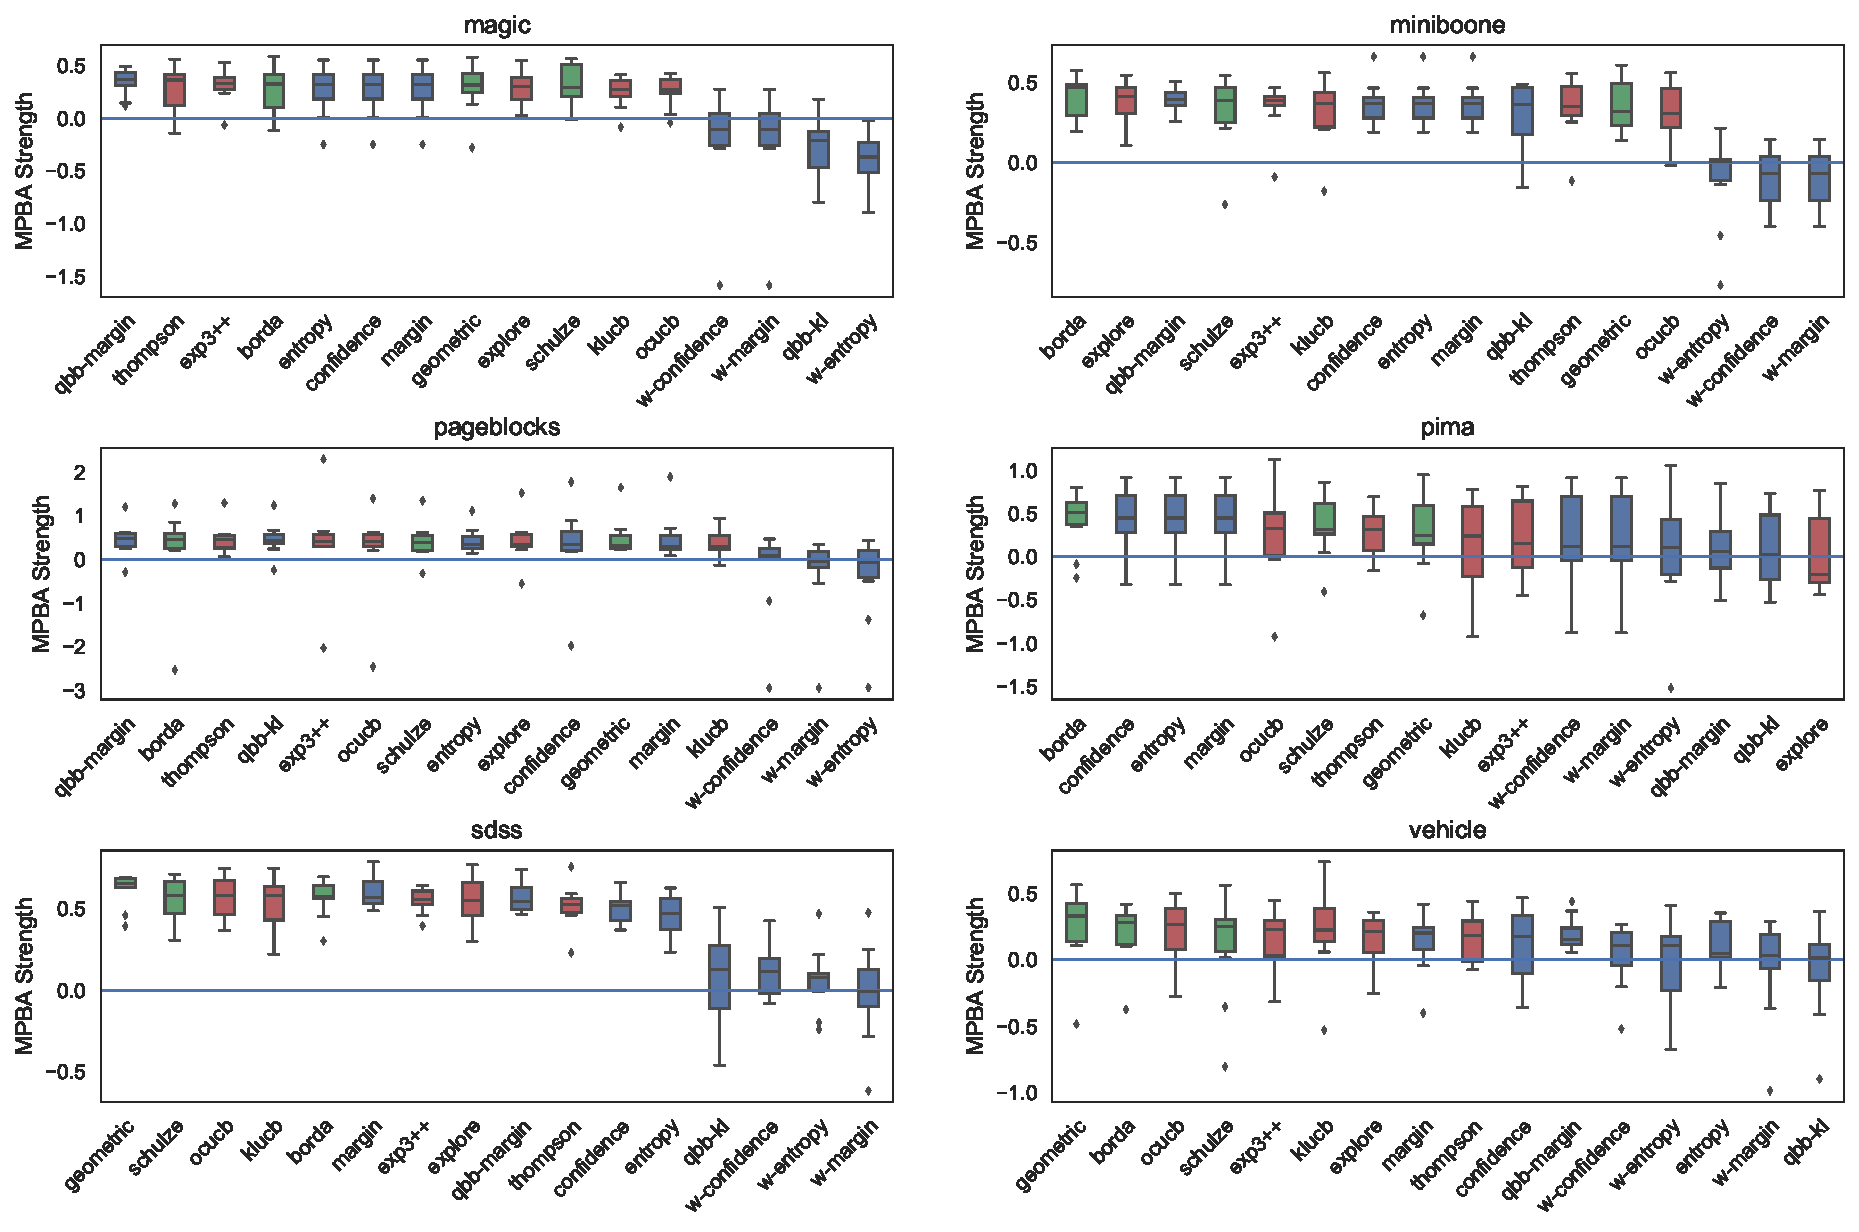
\includegraphics[width=\textwidth]{figures/strengths-mpba-large}
        \caption{Large datasets}
    \end{subfigure}
	\caption[Policy strength]{Boxplots of MPBA strength of policies and
	heuristics relative to passive learning. The more positive the strength is,
	the better the heuristic/policy. Blue boxes represent individual
	heuristics; red boxes represent bandit alogrithms, and green boxes are for
	rank aggragation algorithms. Each plot is over 10 trials.}
	\label{fig:strengths-mpba}
\end{figure}


\begin{figure}[tbp]
	\centering
	\begin{subfigure}[t]{\textwidth}
        \centering
        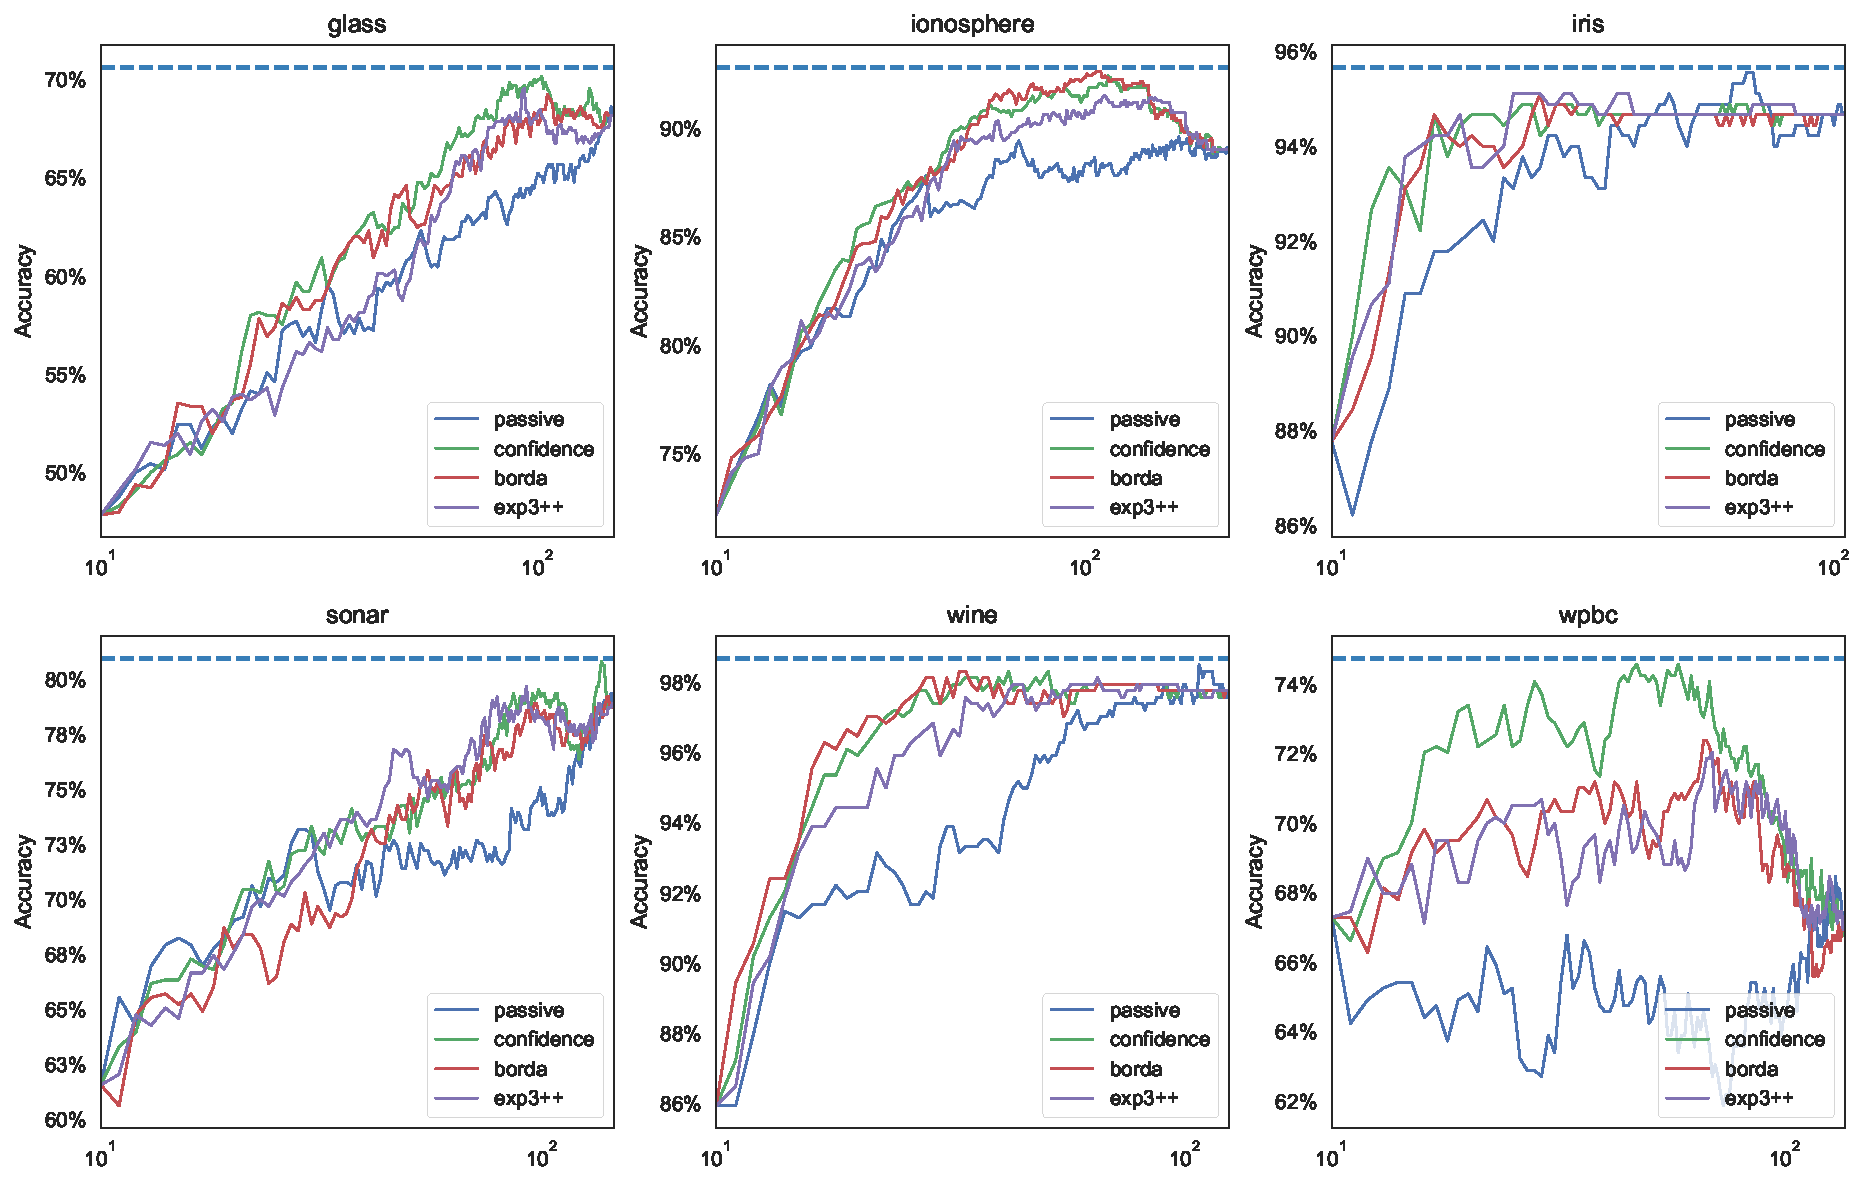
\includegraphics[width=\textwidth]{figures/learning_curves-accuracy-small}
        \caption{Small datasets}
	\end{subfigure}
	\begin{subfigure}[t]{\textwidth}
        \centering
        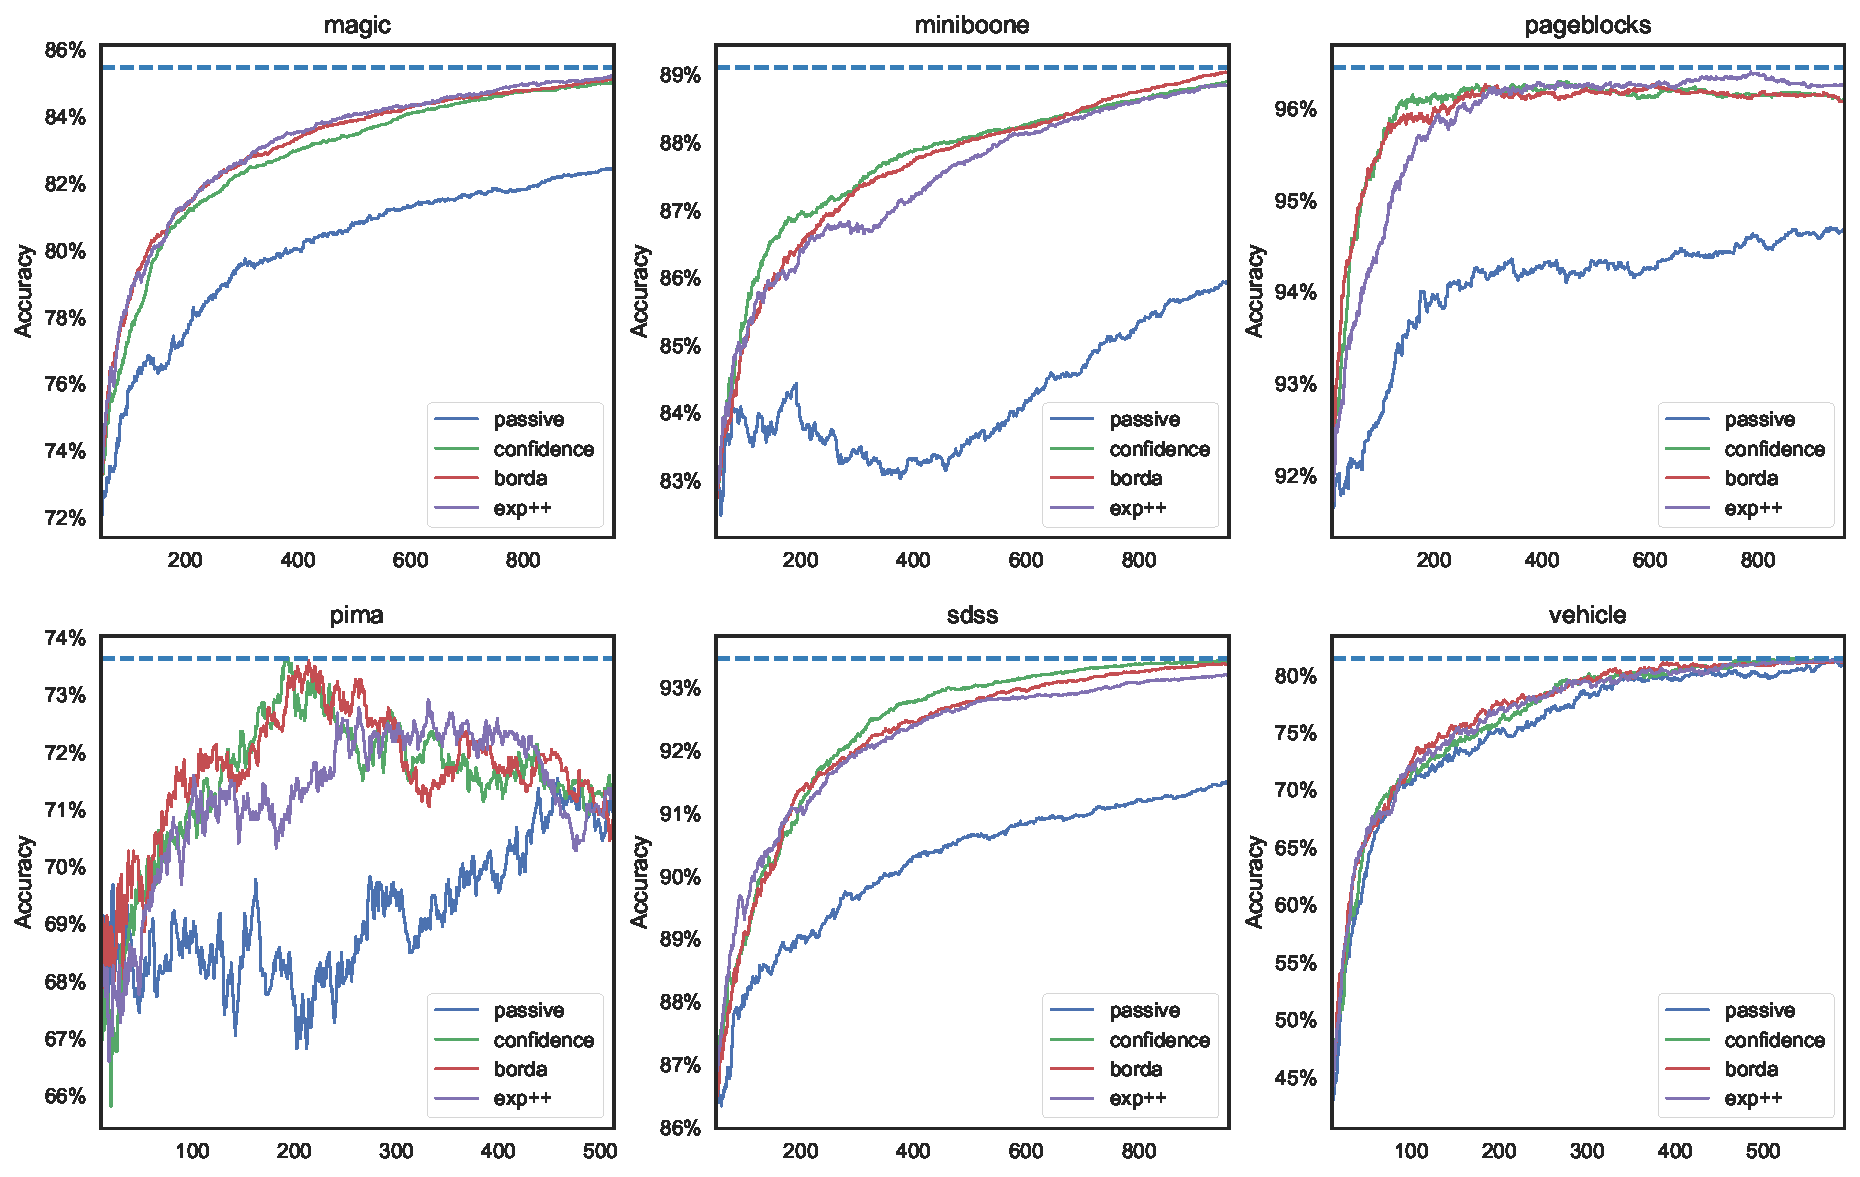
\includegraphics[width=\textwidth]{figures/learning_curves-accuracy-large}
        \caption{Large datasets}
    \end{subfigure}
	\caption[Selected learning curves]{Selected accuracy rate learning curves.
	As it would get too cluttered to plot 16 learning curves, we only show the
	MPBA curves for the least confidence heuristic, the EXP3++ bandit policy,
	and the Borda aggregation policy. The learning curves are averaged over 10
	shuffles.}
	\label{fig:learning_curves-accuracy}
\end{figure}

\begin{figure}[tbp]
	\centering
	\begin{subfigure}[t]{\textwidth}
        \centering
        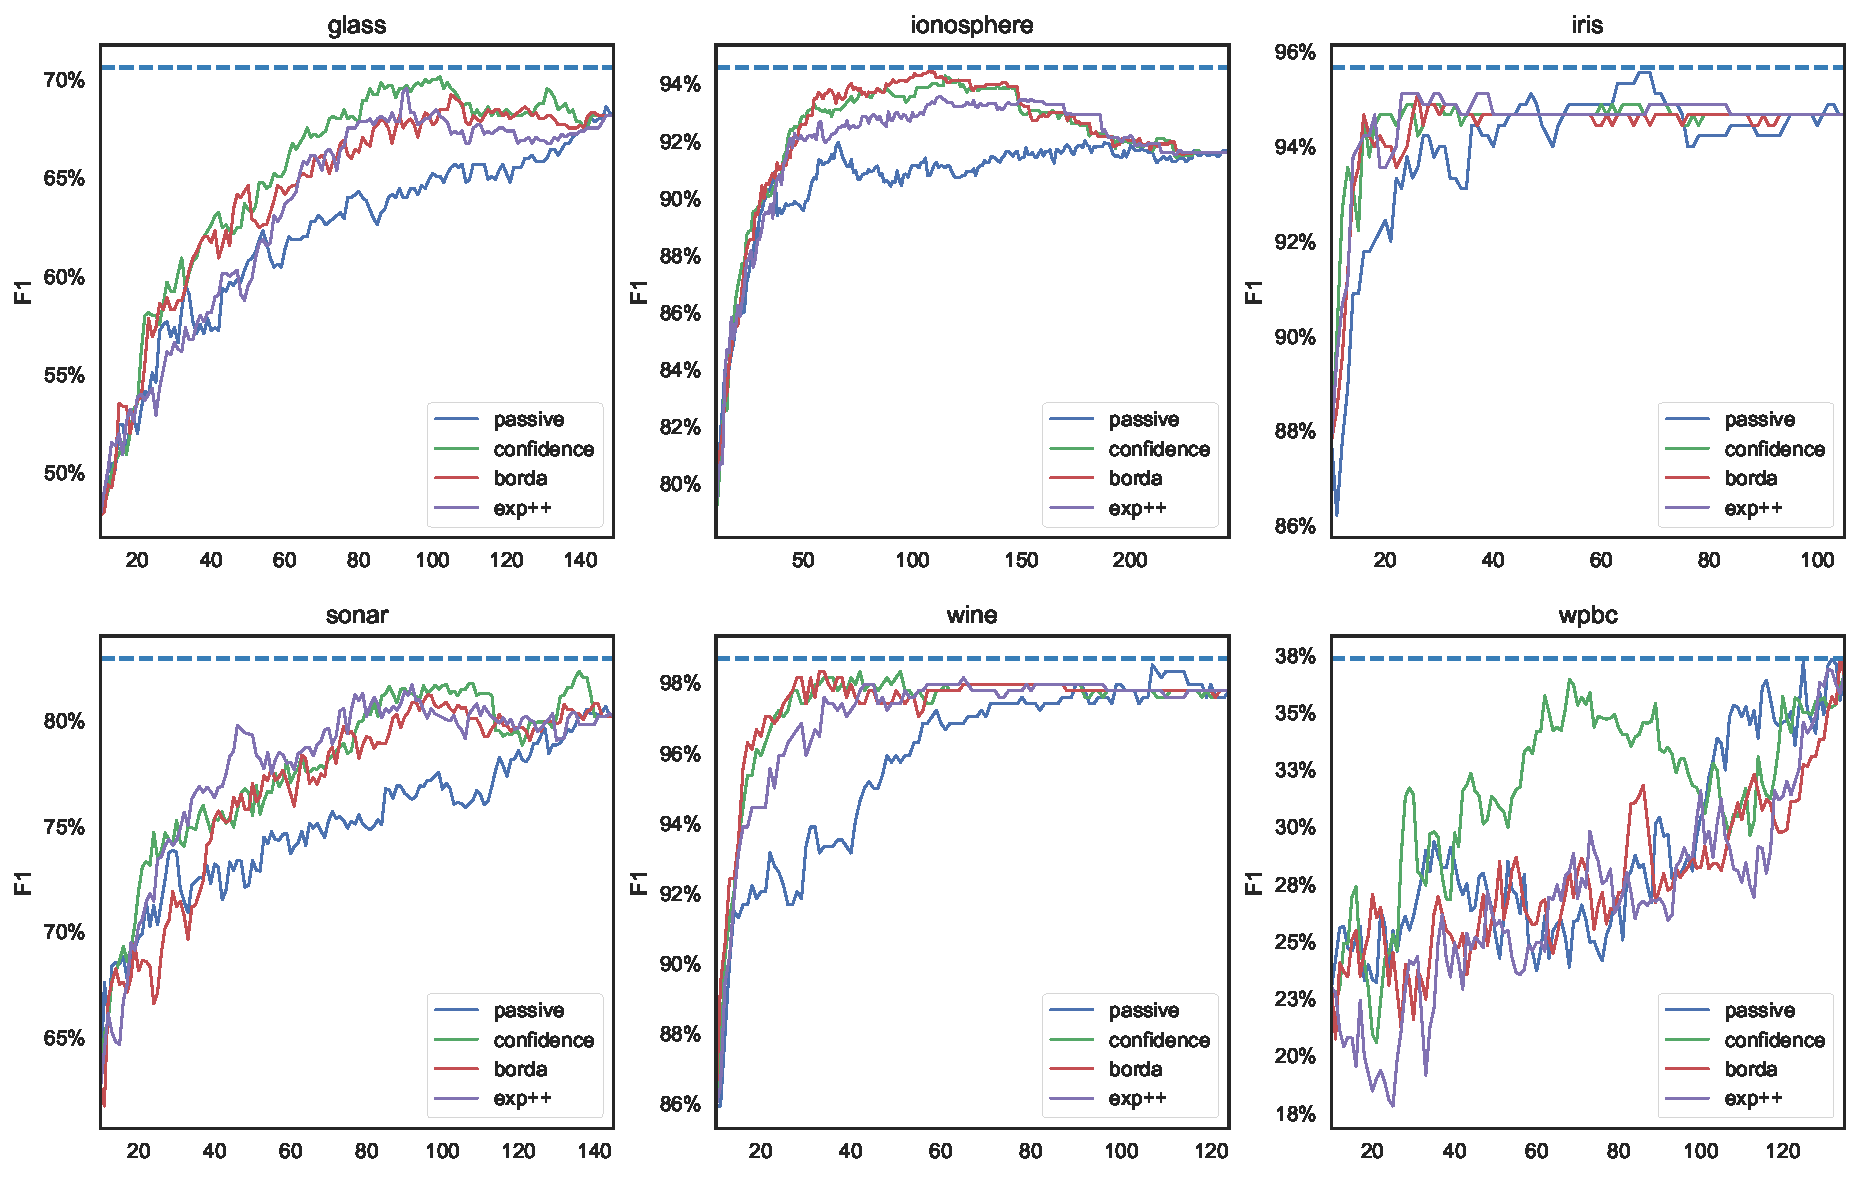
\includegraphics[width=\textwidth]{figures/learning_curves-f1-small}
        \caption{Small datasets}
	\end{subfigure}
	\begin{subfigure}[t]{\textwidth}
        \centering
        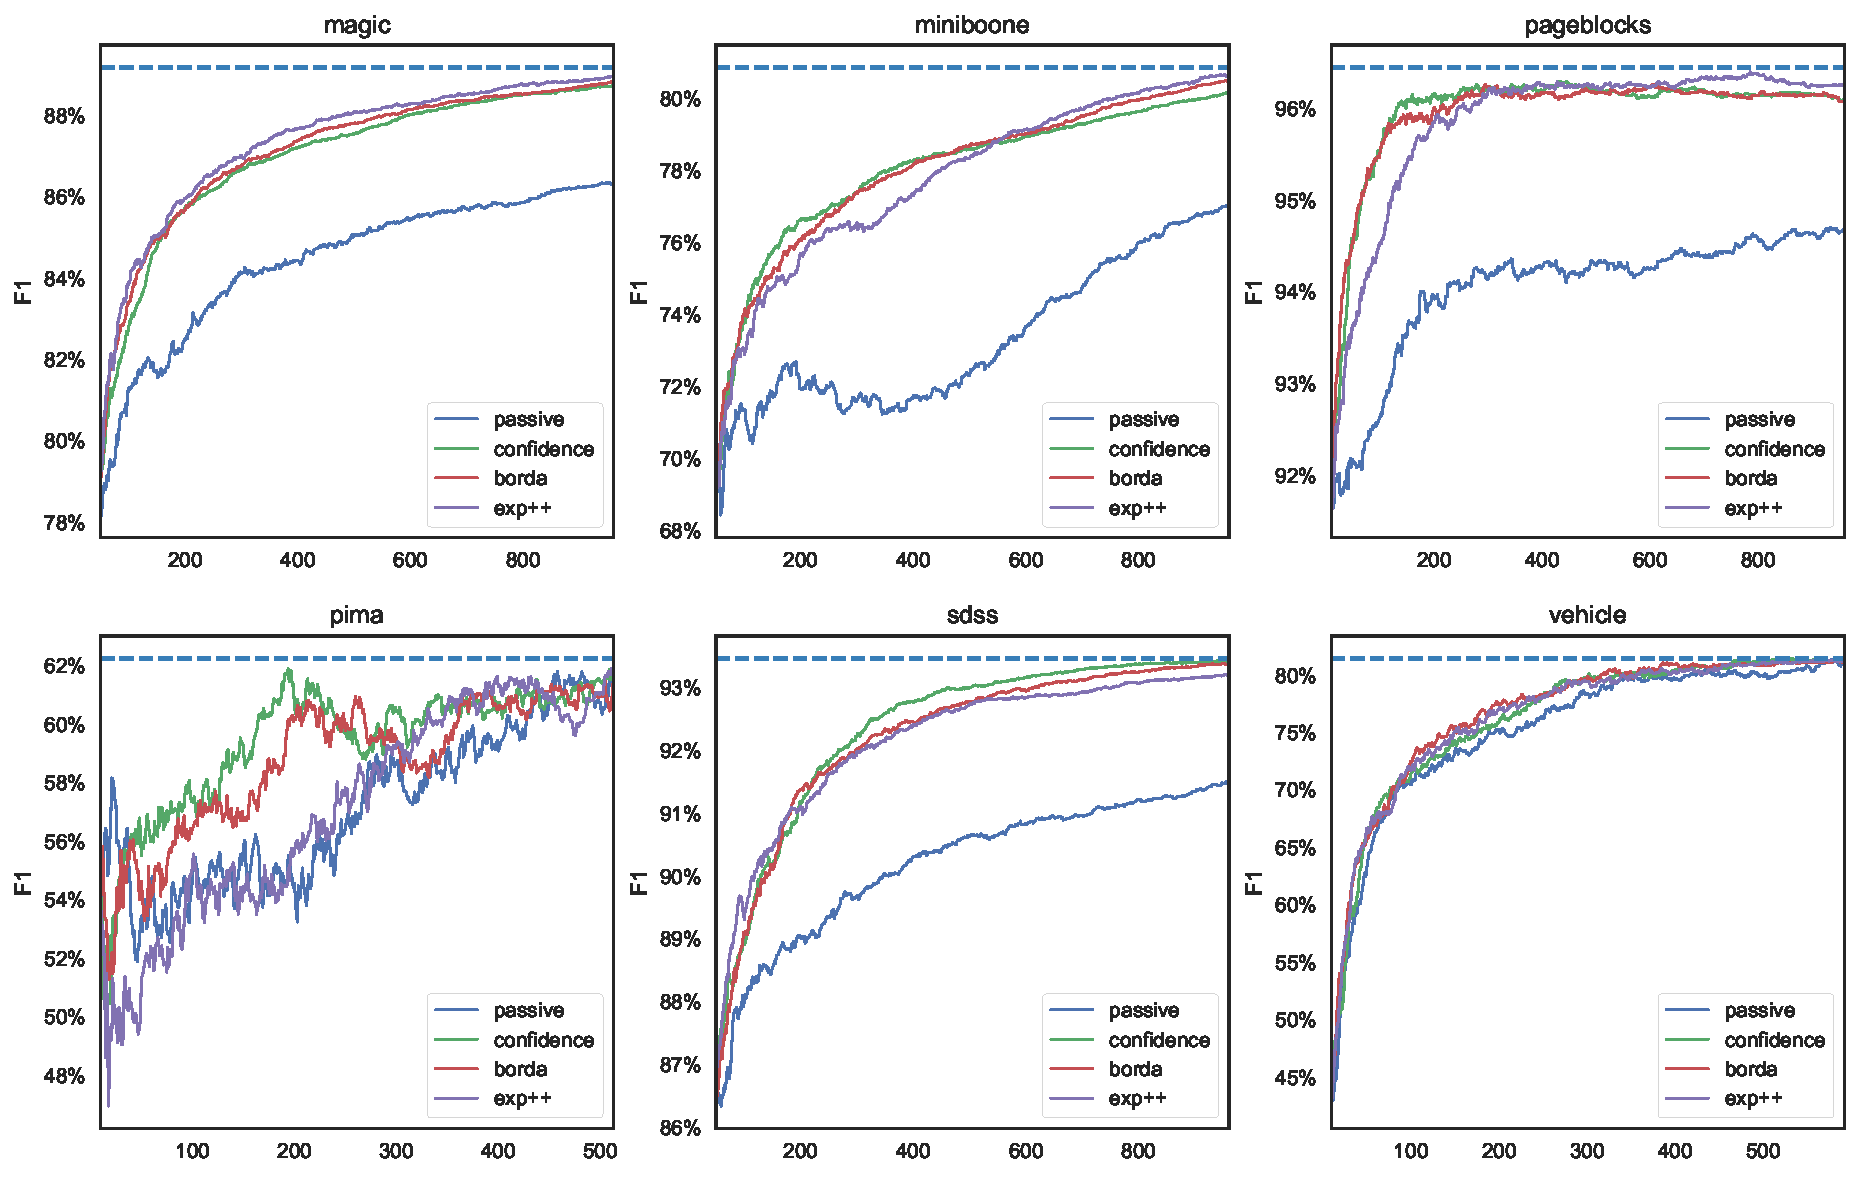
\includegraphics[width=\textwidth]{figures/learning_curves-f1-large}
        \caption{Large datasets}
    \end{subfigure}
	\caption[Selected learning curves]{Selected F1-score learning curves.
	As it would get too cluttered to plot 16 learning curves, we only show the
	MPBA curves for the least confidence heuristic, the EXP3++ bandit policy,
	and the Borda aggregation policy. The learning curves are averaged over 10
	shuffles.}
	\label{fig:learning_curves-f1}
\end{figure}

\begin{figure}[tbp]
	\centering
	\begin{subfigure}[t]{\textwidth}
        \centering
        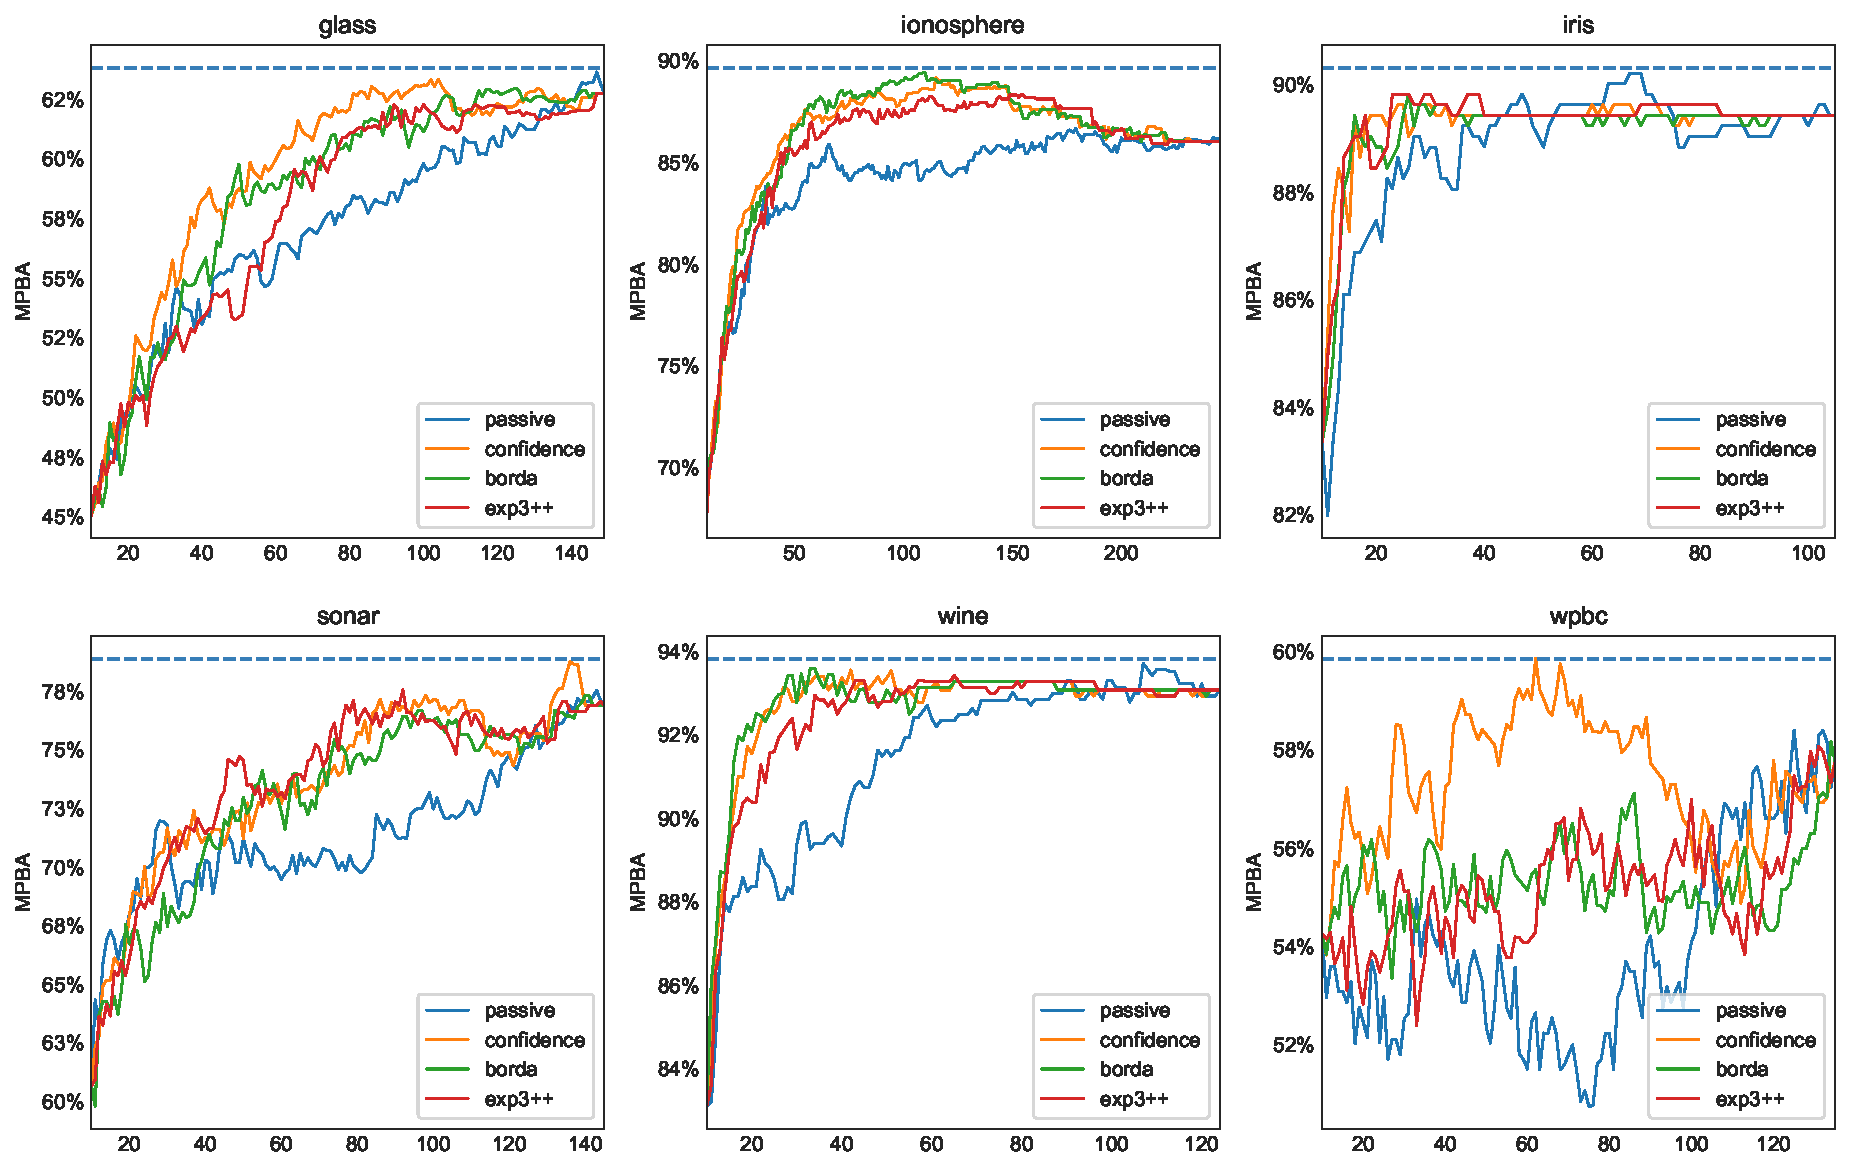
\includegraphics[width=\textwidth]{figures/learning_curves-mpba-small}
        \caption{Small datasets}
	\end{subfigure}
	\begin{subfigure}[t]{\textwidth}
        \centering
        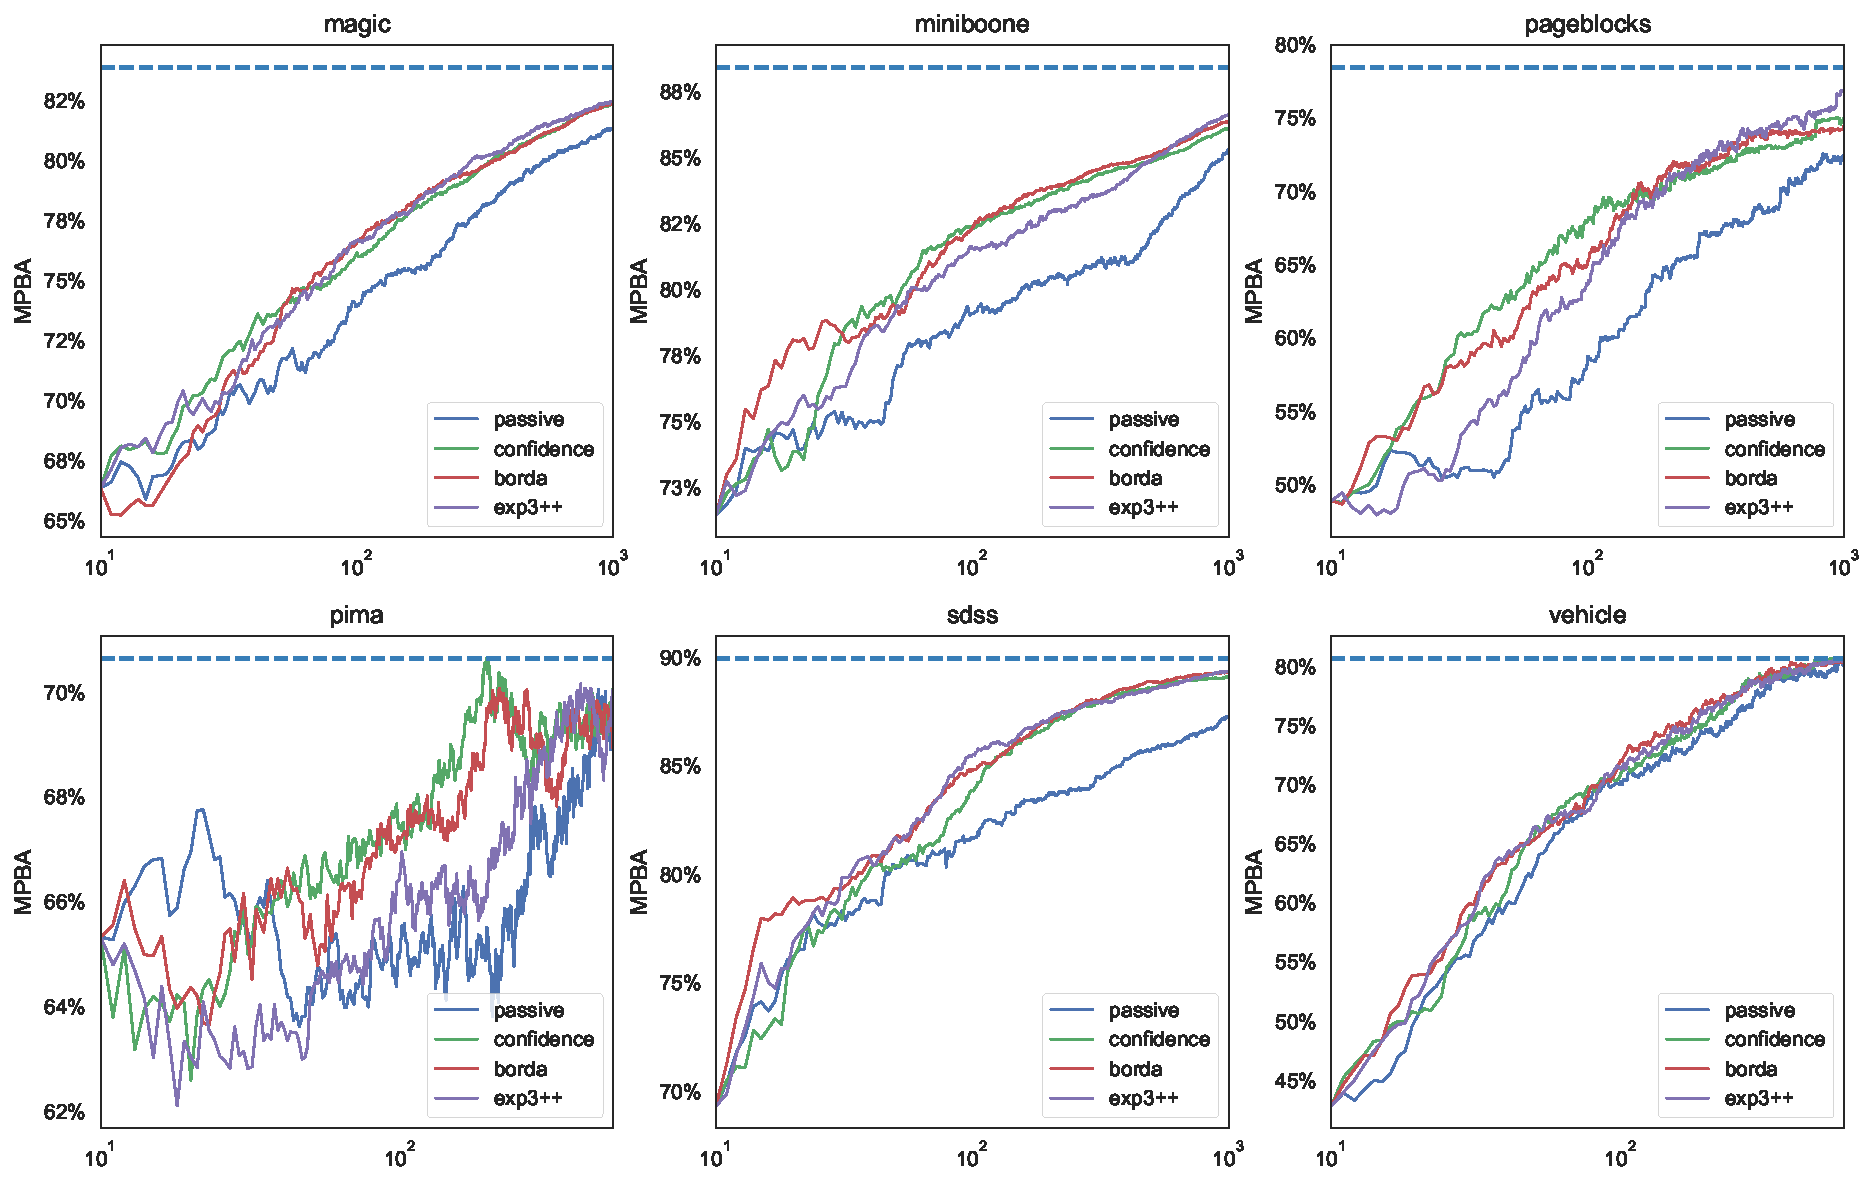
\includegraphics[width=\textwidth]{figures/learning_curves-mpba-large}
        \caption{Large datasets}
    \end{subfigure}
	\caption[Selected learning curves]{Selected MPBA learning curves.
	As it would get too cluttered to plot 16 learning curves, we only show the
	MPBA curves for the least confidence heuristic, the EXP3++ bandit policy,
	and the Borda aggregation policy. The learning curves are averaged over 10
	shuffles.}
	\label{fig:learning_curves-mpba}
\end{figure}


\section{Acknowledgments}

Funding for SDSS-III has been provided by the Alfred P. Sloan Foundation, the
Participating Institutions, the National Science Foundation, and the U.S.
Department of Energy Office of Science. The SDSS-III web site is
http://www.sdss3.org/.

SDSS-III is managed by the Astrophysical Research Consortium for the
Participating Institutions of the SDSS-III Collaboration including the
University of Arizona, the Brazilian Participation Group, Brookhaven National
Laboratory, Carnegie Mellon University, University of Florida, the French
Participation Group, the German Participation Group, Harvard University, the
Instituto de Astrofisica de Canarias, the Michigan State/Notre Dame/JINA
Participation Group, Johns Hopkins University, Lawrence Berkeley National
Laboratory, Max Planck Institute for Astrophysics, Max Planck Institute for
Extraterrestrial Physics, New Mexico State University, New York University,
Ohio State University, Pennsylvania State University, University of Portsmouth,
Princeton University, the Spanish Participation Group, University of Tokyo,
University of Utah, Vanderbilt University, University of Virginia, University
of Washington, and Yale University.



\bibliography{active}

\pagebreak

\section*{Appendix A: Posterior Balanced Accuracy}


Most real-world datasets are unbalanced. In the SDSS dataset, for example,
there are 4.5 times as many galaxies as quasars. The problem of class imbalance
is even more severe in the pageblock dataset, where one class makes up 90\% of
the data and the remaining four classes only make up the remaining 10\%. An
easy fix is to undersample the dominant class when creating training and test
sets. This, of course, means that the size of these sets are limited by the
size of the minority class.

When we do not want to alter the underlying class distributions or when larger
training and test sets are desired, we need a performance measure that can
correct for the class imbalance.~\cite{brodersen10} show that the posterior
balanced accuracy distribution can overcome the bias in the binary case. We now
extend this idea to the multi-class setting.

Suppose we have $k$ classes. For each class $i$ between $1$ and $k$, there are
$N_i$ objects in the universe. Given a classifier, we can predict the label of
every object and compare our prediction to the true label. Let $G_i$ be the
number of objects in class $i$ that are correctly predicted.
Then we define the recall $A_i$ of class $i$ as\index{recall}
	\begin{IEEEeqnarray}{lCl}
		A_i &=& \frac{G_i}{N_i}
	\end{IEEEeqnarray}
The problem is that it is not feasible to get the actual values of $G_i$ and
$N_i$ since that would require us to obtain the true label of every object.
Thus we need a method to estimate these quantities when we only have a sample.
Initially we have no information about $G_i$ and $N_i$, so we can assume that
each $A_i$ follows a uniform prior from 0 to 1. This is the same as a Beta
distribution with shape parameters $\alpha = \beta = 1$:
	\begin{IEEEeqnarray}{lCl}
		A_i &\sim& \Beta(1,1)
	\end{IEEEeqnarray}
The PDF of $A_i$ is then
    \begin{IEEEeqnarray}{lCl}
        f_{A_i}(a) &=& \frac{\Gamma(\alpha+\beta)}{\Gamma(\alpha)\Gamma(\beta)}\,
        a^{\alpha-1}(1-a)^{\beta-1} \label{eqn:prior} \\
        &\propto&   a^{1-1}(1-a)^{1-1}  \notag
    \end{IEEEeqnarray}
where $\Gamma(\alpha)$ is the gamma function.

After we have trained the classifier, suppose we have a test set containing
$n_i$ objects in class $i$. Running the classifier on this test set is the same
as conducting $k$ binomial experiments, where, in the $i$th experiment, the
sample size is $n_i$ and the probability of success is simply $A_i$. Let $g_i$
be the number of correctly labeled objects belonging to class $i$ in the test
set. Then, conditional on the accuracy rate, $g_i$ follows a binomial
distribution:
	\begin{IEEEeqnarray}{lCl}
		(g_i \mid A_i) &\sim& \Bin(n_i, A_i)
	\end{IEEEeqnarray}
The probability mass function of $(g_i \mid A_i = a)$ is thus
    \begin{IEEEeqnarray}{lCl}
		p_{g_i \mid A_i}(g_i) &=& \binom{n_i}{g_i} a^{g_i} (1 - a)^{n_i - g_i}
						  							\label{eqn:likelihood} \\
                              &\propto& a^{g_i} (1 - a)^{n_i - g_i} \notag
    \end{IEEEeqnarray}
In the Bayesian \index{Bayesian} setting,~\eqref{eqn:prior} is the prior and
\eqref{eqn:likelihood} is the likelihood. To get the posterior PDF, we simply
multiply the prior with the likelihood:
	\begin{IEEEeqnarray}{lCl}
		f_{A_i \mid \bm{g}}(a)
		&\propto& f_{A_i}(a) \times f_{g_i \mid A_i}(g_i) \\
		&\propto& a^{1-1}(1-a)^{1-1} \times a^{g_i} (1 - a)^{n_i - g_i} \\
		&=& a^{1 + g_i - 1}(1-a)^{1 + n_i - g_i - 1}
	\end{IEEEeqnarray}
Thus, with respect to the binomial likelihood function,
the Beta distribution is conjugate to itself. The posterior recall rate $A_i$
also follows a Beta distribution, now with parameters
	\begin{IEEEeqnarray}{lCl}
		(A_i \mid g_i) &\sim& \Beta(1 + g_i, 1 + n_i - g_i)
	\end{IEEEeqnarray}
Our goal is to have a balanced accuracy rate, $A$, that puts an equal weight in
each class. One way to achieve this is to take the average of the individual
recalls:
	\begin{IEEEeqnarray}{lCl}
		A &=& \frac{1}{k} \sum_{i=1}^k A_i \\
		&=& \frac{1}{k} A_T
	\end{IEEEeqnarray}
Here we have defined $A_T$ to be the sum of the individual recalls. We call
$(A \mid \bm{g})$ the posterior balanced accuracy (PBA), where $\bm{g}
=(g_1,...,g_k)$. Most of the time, we simply want to calculate its expected
value:
	\begin{IEEEeqnarray}{lCl}
		\E{A \given \bm{g}} &=& \frac{1}{k} \, \E{A_T \given \bm{g}} \\
		&=& \frac{1}{k} \int a \cdot f_{A_T \mid \bm{g}}(a) \, da
	\end{IEEEeqnarray}
Let us call this the mean posterior balanced accuracy (MPBA). Note that there
is no closed form solution for the PDF $f_{A_T \mid \bm{g}}(a)$. However
assuming that $A_T$ is a sum of $k$ independent Beta random variables, $f_{A_T
\mid \bm{g}}(a)$ can be approximated by numerically convolving $k$ Beta
distributions. The independence assumption is reasonable here, since there
should be little to no correlation between the individual class accuracy rates.
Knowing that a classifier is really good at recognising stars does not tell us
much about how well that classifier can recognise galaxies.

Having the knowledge of $f_{A \mid \bm{g}}(a)$ will allow us to make violin
plots, construct confidence intervals and do hypothesis tests. To get an
expression for this, let us first rewrite the cumulative distribution function
(CDF) as
	\begin{IEEEeqnarray}{lCl}
		F_{A\mid \bm{g}}(a) &=& \Prob{A \leq a \mid \bm{g}} \\
		&=& \Prob[\Big]{\frac{1}{k} A_T \leq a \given \bm{g}} \\
		&=& \Prob{A_T \leq ka \given \bm{g}} \\
		&=& F_{A_T \mid \bm{g}}(ka) \IEEEyesnumber \label{eqn:CDF}
	\end{IEEEeqnarray}
Differentiating \eqref{eqn:CDF} with respect to $a$, we obtain the PDF of $(A \mid \bm{g})$:
	\begin{IEEEeqnarray}{lCl}
		f_{A \mid \bm{g}}(a) &=& \frac{\partial}{\partial a} F_{A \mid \bm{g}}(ka) \\
		&=& \frac{\partial}{\partial a} (ka) \cdot \frac{\partial}{\partial ka}
			F_{A_T \mid \bm{g}}(ka) \\
		&=& k \cdot f_{A_T \mid \bm{g}}(ka)
	\end{IEEEeqnarray}

\end{document}
